\documentclass[11pt]{article}
\usepackage{times}
\usepackage{amsmath,amsthm,amssymb,setspace,enumitem,epsfig,titlesec,verbatim,color,array,eurosym,multirow}
\usepackage[sort&compress]{natbib}
\usepackage[footnotesize,bf]{caption}
\usepackage[margin=2.5cm, includefoot, footskip=30pt]{geometry}
\usepackage{standalone}
\usepackage{tikz}
\usepackage{subcaption}
\usepackage{hyperref}
\usepackage{tabularx}
\usepackage{booktabs}
\usepackage{blkarray}
\usepackage[ruled,vlined]{algorithm2e}
\smallskip % Erlaubt kleine Abstaende zwischen Paragraphen, falls es dem Seitenlayout hilft
\renewcommand{\baselinestretch}{1.3}
\newcommand{\R}{\mathbb{R}}

\definecolor{darkblue}{rgb}{0,0,.8}
\definecolor{darkgreen}{rgb}{0,0.5,0.1}
\newcommand{\matlabfunc}[1]{\textcolor{darkblue}{#1}}
\newcommand{\matlabcomment}[1]{\textcolor{darkgreen}{#1}}
\newcommand{\christian}[1]{\textcolor{blue}{\textbf{CH}: #1}}
\newcommand{\alex}[1]{\textcolor{red}{\textbf{AL}: #1}}

%% Adding shortcut commands to refer to our figures %%
\newcommand{\FigEvoProc}{{\bf Fig.~1}} \newcommand{\FigInvAnalysis}{{\bfFig.~2}} \newcommand{\FigResultsOverPara}{{\bf Fig.~3}}


\titleformat{\section}{\sffamily \fontsize{12}{14}\bfseries}{\thesection}{1em}{}
\titleformat{\subsection}{\sffamily
\fontsize{11.5}{11.5}\bfseries}{\thesubsection}{1em}{}

\usepackage{tikz}
\usetikzlibrary{arrows}

\tikzset{treenode/.style = {align=center, inner sep=0pt, text centered,
  font=\sffamily}, arn_n/.style = {treenode, circle, white,
  font=\sffamily\bfseries, draw=black, inner sep=-6pt, fill=black, text
  width=1.5em},% arbre rouge noir, noeud noir
  arn_r/.style = {treenode, circle, red, text width=1.5em, very thick, inner
    sep=4pt},% arbre rouge noir, noeud rouge
  arn_x/.style = {treenode, rectangle, draw=black, minimum width=0.5em, minimum
    height=0.5em}% arbre rouge noir, nil
}

\newtheoremstyle{plainCl1}% name
{9pt}%      Space above, empty = 'usual value'
{9pt}%      Space below
{\it}% 	   Body font
{}%         Indent amount (empty = no indent, \parindent = para indent)
{\bfseries}% Thm head font
{.}%        Punctuation after thm head
{0.2cm}% Space after thm head: \newline = linebreak
{}%         Thm head spec

\newtheoremstyle{plainCl2}% name
{9pt}%      Space above, empty = 'usual value'
{9pt}%      Space below
{\it}% 	   Body font
{}%         Indent amount (empty = no indent, \parindent = para indent)
{\bfseries}% Thm head font
{$'$.}%        Punctuation after thm head
{0.2cm}% Space after thm head: \newline = linebreak
{}%         Thm head spec

\newcommand{\splitatcommas}[1]{%
  \begingroup
  \begingroup\lccode`~=`, \lowercase{\endgroup \edef~{\mathchar\the\mathcode`,
    \penalty0 \noexpand\hspace{0pt plus 1em}}%
  }\mathcode`,="8000 #1%
  \endgroup
}

\theoremstyle{plainCl1}
\newtheorem{Claim}{Claim}
\newtheorem{Thm}{Theorem}
\newtheorem{Prop}{Proposition}
\newtheorem*{Lem}{Lemma}
\newtheorem{Cor}{Corollary}
\newtheorem*{Def}{Definition}

\theoremstyle{plainCl2}
\newtheorem{Claim2}{Claim}

\title{\bf  \sffamily \LARGE Evolution of cooperation among individuals with
limited payoff memory\\}
\date{}
\author{Nikoleta E. Glynatsi, Christian Hilbe, Alex McAvoy}

\begin{document}
\maketitle

\begin{abstract}
Repeated games are vastly used in evolutionary game theory to explain cooperation
in a variety of environments. Although existing models have shaped our
understanding of human cooperation they often work with idealized assumptions.
In an evolutionary process, individuals imitate other individuals of the
population based on their fitness. It is commonly assumed that an individual
computes their fitness after interacting with a representative sample of the
population and remembering all the interactions they participated in. In real
life we do not always remember all our interactions, instead we rather recall
our most recent ones.

Here we introduce a framework that allows individuals to estimate their fitness
based on a minimum of social information. We explore the difference between our
framework and the classical framework using computer simulations. The
simulations show that in the prisoner's dilemma, individuals with limited memory
tend to adopt less generous strategies and they achieve less cooperation than in
the classical scenario.
\end{abstract}

\section{Introduction}

Evolutionary game theory~\cite{smith1982evolution, hofbauer1998evolutionary,
nowak:Nature:2004, hauert2005game} describes the evolutionary dynamics of
populations consisting of different types of interacting individuals. In the
last two decades the interest of the field has shifted to the analysis of
stochastic finite population dynamics in preference to traditional approaches
such as the replicator dynamics~\cite{hofbauer:JTB:1979, taylor:MATHBIO:1978}.
This is especially true in the topic of cooperation~\cite{hilbe:PNAS:2013,
hilbe:Nature:2018,glynatsi:SCR:2020}. In stochastic evolutionary dynamics
disadvantageous mutants have a small yet non-zero probability to reach fixation
and this can lead to fundamental changes in the results. As shown
in~\cite{nowak:Nature:2004}, using such dynamics a single cooperative strategy
can invade a population of defectors without any special modifications in
comparison to traditional approaches that one has to consider spatial
structure~\cite{nowak:Nature:1992} or when payoffs are subject to aggregate
shocks~\cite{fudenberg:JET:1992}.

Stochastic evolutionary dynamics model a finite population. Each
time step of the process consists of three phases; (1) the \textit{mutation
phase} (2) the \textit{game phase} (3) the \textit{update phase}. In the
mutation phase one individual from the population is chosen to switch to a new
mutant strategy with a probability \(\mu\). In the game phase individuals are
randomly matched with other individuals in the population, and they engage in a
repeated game where each subsequent turn occurs with a fixed probability
\(\delta\). The updating phase depends on the process. Two classes of
finite stochastic processes have been used extensively: (i) fitness-based
processes in which an individual chosen proportional to fitness reproduces and
the offspring replaces a randomly chosen individual~\cite{nowak:Nature:2004} or
(ii) \textit{pairwise comparison processes} in which a pair of individuals is
chosen and subsequently one of these individuals may adopt the strategy of the
other~\cite{traulsen2007pairwise}.

Similar to all other theoretical models, finite stochastic processes rest on a
set of assumptions. Namely, in the game phase it is assumed that players use
strategies with finite memory~\cite{Nowak1992tit, Baek2016}. For example, in a
repeated game between two individuals the actions of the players in each turn
are often determined by the action of the co-players in the previous turn. This
assumption is common as it allows for an explicit calculation of the players'
payoffs~\cite{sigmund2010calculus}. In addition, it is
assumed that individuals play many times and with all other players before
reproduction takes place. So that in the updating phase the updating payoffs, and
subsequently the fitness, of individuals is given by the average payoffs of an
infinitely repeated game against the mean distribution of types in the
population.

The above two assumptions create a curious inconsistency; a player with a finite
memory in the game stage can recall infinite information regarding their
interactions and each interaction's outcomes in the update stage. Previous work
has explored the effects of constraining the interactions an individual has.
Either by letting individuals have a stochastic number of
interactions~\cite{roca:PhysicalReview:2006, sanchez:JTB:2005,
Traulsen:JTB:2007} or by only allowing for
a single interaction~\cite{Woelfing:JTB:2009}. However, no previous work
considers that not only the interactions are limited but also the information
regarding each interaction. To this end, we propose a framework in which
individuals, similar to the decisions at each turn, estimate their fitness based
on a minimum of information.

We first consider two extreme scenarios, the classical scenario where an individual
has a perfect memory of all their interactions and the alternative scenario of
limited memory where individuals update their strategies only based on the very
last payoff they obtained. We demonstrate the effects of limited payoff
memory using a pairwise comparison process and the well studied game of the
prisoner's dilemma. We observe that individuals with limited payoff memory tend to
adopt less generous strategies and they achieve less cooperation when
interacting in a prisoner's dilemma. We obtain similar results when we consider
that individuals update their strategies based on more information. More
specifically, up to the last two payoffs they obtained when interacting with up
to two different members of the population.

\section{Model Setup}\label{section:model}

A pairwise comparison process starts with assigning all
individuals of the population the same strategy. Each elementary time step of
the process consists of the mutation phase, the game phase and the update phase.
In the game phase individuals are matched in pairs and that they participate in
a repeated 2 person donation game; a special case of the prisoner's dilemma. In
the donation game there are two actions: cooperation (\(C\)) and defection
(\(D\)). By cooperating a player provides a benefit \(b\) to the other player at
their cost \(c\), with \(0 < c < b\). Thus the payoffs for a player in each turn
are,

\begin{equation}
    \begin{blockarray}{ccc}
        & \text{cooperate} & \text{defect} \\
        \begin{block}{c(cc)}
            \text{cooperate} & b - c & -c \\
            \text{defect} & b & 0 \\
        \end{block}
    \end{blockarray}.
\end{equation}

Let \(\mathbf{u} = (b-c, -c, b, 0)\) be payoffs in a vector format, and let
\(\mathcal{U} = \{r, s, t, p\}\) denote the set of feasible payoffs, where \(r\)
denotes the payoff of mutual cooperation, \(s\) the sucker's payoff, \(t\) the
temptation to defect payoff, and \(p\) the punishment payoff.

In repeated games there are infinite many strategies, however, similar to the
literature we will assume that individuals use reactive strategies. A reactive
strategy considers only the previous action of the other player, and thus, a
reactive strategy \(s\) can be written as a three-dimensional vector \(s=(y, p,
q)\). The parameter \(y\) is the probability that the strategy opens with a
cooperation and \(p\), \(q\) are the probabilities that the strategy cooperates
given that the opponent cooperated and defected equivalently. The play between a
pair of reactive strategies ($s_1 = (y_1, p_1, q_1)$, $s_2 = (y_2, p_2, q_2)$)
can be model as a Markov process with the transition matrix \(M\),

\begin{equation}\label{eq:transition_matrix}
  M = \left[\begin{matrix} p_{1} p_{2} & p_{1} \left(1 - p_{2}\right) & p_{2} \left(1 - p_{1}\right) & \left(1 - p_{1}\right) \left(1 - p_{2}\right)\\
    p_{2} q_{1} & q_{1} \left(1 - p_{2}\right) & p_{2} \left(1 - q_{1}\right) & \left(1 - p_{2}\right) \left(1 - q_{1}\right)\\
    p_{1} q_{2} & p_{1} \left(1 - q_{2}\right) & q_{2} \left(1 - p_{1}\right) & \left(1 - p_{1}\right) \left(1 - q_{2}\right)\\
    q_{1} q_{2} & q_{1} \left(1 - q_{2}\right) & q_{2} \left(1 - q_{1}\right) & \left(1 - q_{1}\right) \left(1 - q_{2}\right)\end{matrix}\right]
\end{equation}

and the stationary vector \(\mathbf{v}(s_1,s_2)\)
which is the solution to \(\mathbf{v}(s_1,s_2) \times M 
= \mathbf{v}(s_1,s_2)\).

In the update stage two individuals are randomly selected. From the two
individuals, one  serves as the `learner' and the other as the `role model'. The
learner adopts the role model's strategy with a probability \(\rho\) given by,

\begin{equation} \label{Eq:rho}
    \rho(\pi_{L}, \pi_{RM}) = \frac{1}{1\!+\! e^{\!-\!\beta (\pi_{RM}\!-\! \pi_{L})}}.
\end{equation}

\(\pi_{L}\) and \(\pi_{RM}\) are the updating payoffs/fitness of the learner and the
role model respectively. The updating payoffs are a measure of how successful
individuals are in the current standing of the population. The parameter
\(\beta\) is known as the selection strength, namely, it shows how important the
payoff difference is when the learner is considering adopting the strategy of
the role model.

For the results presented here we assume that mutations are rare (\(\mu
\rightarrow 0\)). In fact, so rare that only two different strategies can be
present in the population at any given time. However, in the Supplementary Information
Section 4 we show in that the main result hold for \(\mu \neq 0\).
The case of low mutation is vastly adopted because it allows us to explicitly
calculate the fixation probability of a newly introduced mutant. More specifically,
at each step
one individual adopts a mutant strategy randomly selected from the set of
feasible strategies. The fixation probability \(\phi_{M}\) of the mutant
strategy can be calculated explicitly,

\begin{equation}\label{eq:appendix_fixation_probability}
    \varphi_{M} = \frac{1}{1+\sum\limits_{i=1}^{N-1}\prod\limits_k^i \frac{\lambda^-_k}{\lambda^+_k}},
\end{equation}

where \(\lambda^-_k, \lambda^+_k\) are the probabilities that the number of
mutants decreases and increases respectively, and \(k\) is the number of
mutants. Depending on the fixation probability \(\phi_{M}\) the mutant either
fixes (becomes the new resident) or goes extinct. Regardless, in the elementary
time step another mutant strategy is introduced to the population. We iterate
this elementary population updating process for a large number of mutant
strategies and we record the resident strategies at each time step. The
probabilities \(\lambda^-_k \text{ and } \lambda^+_k\) depend on the updating
payoffs of the mutant and the resident strategies. In the next section we
present how they are calculated in the cases of perfect and limited memory.

\subsection{Updating payoffs based Perfect and Limited Memory}

\subsubsection*{Perfect Memory}

In the perfect memory case an individual updates based on the average payoff
against each other member of the population, otherwise as expected payoffs. In
an infinitely repeated game ($\delta \rightarrow 1$) the payoff of a reactive
strategy \(s_1\) against the reactive strategy \(s_2\) can explicitly be
calculated using the stationary vector \(\mathbf{v}\) and the payoffs' vector as
\(\langle\mathbf{v}(s_1,s_2),\mathbf{u}\rangle\). In a population of size \(N\)
there are \(k\) mutants and \(N - k\) residents. We denote the strategies of
a mutant and of a resident as \(s_M =(y_M, p_M, q_M)\) and \(s_R =
(y_R, p_R, q_R)\). The expected payoffs of a resident (\(\pi_R\)) and of a
mutant (\(\pi_M\)) are given by,

\begin{equation} \label{Eq:ExpPay}
  \begin{array}{lcrcr}
  \displaystyle \pi_R & = &\displaystyle \frac{N\!-\!k\!-\!1}{N-1}\cdot \langle\mathbf{v}(s_R,s_R),\mathbf{u}\rangle	&+	&\displaystyle\frac{k}{N-1}\cdot \langle\mathbf{v}(s_R,s_M),\mathbf{u}\rangle,\\[0.5cm]
  \displaystyle \pi_M & = &\displaystyle\frac{N-k}{N-1}\cdot \langle\mathbf{v}(s_M,s_R),\mathbf{u}\rangle&+	&\displaystyle\frac{k-1}{N-1}\cdot \langle\mathbf{v}(s_M,s_M),\mathbf{u}\rangle.\\
  \end{array}
\end{equation}

The probabilities that the number of mutants decreases and increases,
\(\lambda^-_k\) and \(\lambda^+_k\), in the perfect memory case are defined as,

\begin{align}\label{eq:perfect_memory_lambdas}
  \lambda^-_k \!=\!\rho(\pi_M, \pi_R) \quad \text{ and } \quad \lambda^+_k \!=\!\rho(\pi_R, \pi_M).
\end{align}

\subsubsection*{Limited Memory}

In this case of limited memory we initially define the probability that a
reactive strategy receives the payoff $u\!\in\! \mathcal{U}$ in the very last
round of the game. This is given by Proposition~\ref{proposition:last_round}
(see Supplementary Information Section 2.2.1 for proof).

\begin{Prop}\label{proposition:last_round} Consider a repeated game, with
continuation probability $\delta$, between players with reactive strategies
$s_1\!=\!(y_1, p_1, q_1$)  and $s_2\!=\!(y_2,p_2,q_2)$ respectively. Then
the probability that the $s_1$ player receives the payoff $u\!\in\!
\mathcal{U}$ in the very last round of the game is given by
$v_{u}(s_1,s_2)$, as given by Equation~(\ref{Eq:LastRound}).

\begin{equation} \label{Eq:LastRound}
  \setlength{\arraycolsep}{1pt}
  \begin{array}{rcl}

  v_{r}(s_1,s_2) &= &\displaystyle (1\!-\!\delta)\frac{y_1y_2}{1\!-\!\delta^2 l_1 l_2}+\delta \frac{\Big(q_1+l_1\big((1\!-\!\delta)y_2+\delta q_2\big)\Big) \Big(q_2+l_2\big((1\!-\!\delta)y_1+\delta q_1\big)\Big)}
  {\displaystyle(1\!-\!\delta l_1l_2)(1\!-\!\delta^2 l_1 l_2)} \times r,\\[1cm]

  v_{s}(s_1,s_2) &= &\displaystyle (1\!-\!\delta)\frac{y_1\bar{y}_2}{1\!-\!\delta^2 l_1 l_2}+\delta \frac{\Big(q_1+l_1\big((1\!-\!\delta)y_2+\delta q_2\big)\Big) \Big(\bar{q}_2+\bar{r}_2\big((1\!-\!\delta)y_1+\delta p_1\big)\Big)}
  {\displaystyle(1\!-\!\delta l_1l_2)(1\!-\!\delta^2 l_1 l_2)} \times s,\\[1cm]

  v_{t}(s_1,s_2) &= &\displaystyle (1\!-\!\delta)\frac{\bar{y}_1y_2}{1\!-\!\delta^2 l_1 l_2}+\delta \frac{\Big(\bar{q}_1+\bar{r}_1\big((1\!-\!\delta)y_2+\delta p_2\big)\Big) \Big(q_2+l_2\big((1\!-\!\delta)y_1+\delta q_1\big)\Big)}
  {\displaystyle(1\!-\!\delta l_1l_2)(1\!-\!\delta^2 l_1 l_2)} \times t,\\[1cm]

  v_{p}(s_1,s_2) &= &\displaystyle (1\!-\!\delta)\frac{\bar{y}_1\bar{y}_2}{1\!-\!\delta^2 l_1 l_2}+\delta \frac{\Big(\bar{q}_1+\bar{r}_1\big((1\!-\!\delta)y_2+\delta p_2\big)\Big) \Big(\bar{q}_2+\bar{r}_2\big((1\!-\!\delta)y_1+\delta p_1\big)\Big)}
  {\displaystyle(1\!-\!\delta l_1l_2)(1\!-\!\delta^2 l_1 l_2)} \times p.
  \end{array}
\end{equation}

In these expressions, we have used the notation $l_i:=p_i\!-\!q_i$,
$\bar{y}_i\!=\!1\!-\!y_i$, $\bar{q}_i:=1\!-\!q_i$, and
$\bar{l}_i:=\bar{p}_i\!-\!\bar{q}_i=-l_i$ for $i\!\in\!\{1,2\}$.
\end{Prop}

In the case of limited payoffs memory both the role model and the learner
estimate their fitness after interacting with a single member of the population.
At each time step there are five possible pairings. They interact with each
other with a probability \(\frac{1}{N - 1}\), and thus they do not interact with
other with a probability \(1 - \frac{1}{N - 1}\). In the latter case, each of
them can interact with either a mutant or a resident. Both of them interact with
a mutant with a probability $\frac{(k-1)(k-2)}{(N-2)(N-3)}$ and both interact
with a resident with a probability $\frac{(N-k-1)(N-k-2)}{(N-2)(N-3)}$. The last
two possible pairings are that either of them interacts with a resident whilst
the other interacts with a mutant, and this happens with a probability
$\frac{(N-k-1)(k-1)}{(N-2)(N-3)}$. Thus we the probability that the randomly
chosen resident obtained a payoff of $u_R$ in the last round of his respective
game, and that the mutant obtained a payoff of $u_M$ as $x(u_R,u_M)$.

\begin{equation}\label{eq:Chi}
\setlength{\arraycolsep}{1pt}
\begin{array}{llrl}
x(u_1,u_2)	 &=&\displaystyle \frac{1}{N\!-\!1}\cdot  &v_{u_1}(s_1,s_2)\cdot 1_{(u_1,u_2)\in \mathcal{U}^2_F}\\[0.5cm]
&+	
&\displaystyle \left(1\!-\!\frac{1}{N\!-\!1}\right)  
&\left[ \frac{k\!-\!1}{N\!-\!2}\frac{k\!-\!2}{N\!-\!3} v_{u_1}(s_1,s_2) v_{u_2}(s_2,s_2) + 
 \frac{k\!-\!1}{N\!-\!2}\frac{N\!-\!k\!-\!1}{N\!-\!3} v_{u_1}(s_1,s_2) v_{u_2}(s_2,s_1)\right.\\[0.5cm]
&&&\left. +\frac{N\!-\!k\!-\!1}{N\!-\!2}\frac{k\!-\!1}{N\!-\!3} v_{u_1}(s_1,s_1) v_{u_2}(s_2,s_2) + 
 \frac{N\!-\!k\!-\!1}{N\!-\!2}\frac{N\!-\!k\!-\!2}{N\!-\!3} v_{u_1}(s_1,s_1) v_{u_2}(s_2,s_1)\right].
\end{array}
\end{equation}

The first term on the right side corresponds to the case that the learner and
the role model happened to be matched during the game stage, which happens with
probability $\frac{1}{(N\!-\!1)}$. The probability that the number of mutants
increases and decreases by one in the case of limited memory are now given by,

\begin{align}\label{eq:limited_memory_lambdas}
\lambda^+_k=\frac{N\!-\!k}{N} \frac{k}{N} \sum_{u_{R},u_{M}\in\mathcal{U}} x(u_{R},u_{M}) \rho(u_{R},u_{M}) \quad \text{and} \quad
\lambda^-_k=\frac{N\!-\!k}{N} \frac{k}{N} \sum_{u_{R},u_{M}\in\mathcal{U}} x(u_{R},u_{M}) \rho(u_{M},u_{R}).
\end{align}

In this expression, $\frac{(N\!-\!k)}{N}$ is the probability that the randomly
chosen learner is a resident, and $\frac{k}{N}$ is the probability that the role
model is a mutant. The sum corresponds to the total probability that the learner
adopts the role model's strategy over all possible payoffs $u_R$ and $u_M$ that
the two player may have received in their respective last rounds.

\subsubsection*{Simulation Results}

In order to account for the effect of the updating payoffs we simulate the
evolutionary process and record which strategies the players adopt over time
based on perfect memory payoffs and limited memory payoffs. In the case of
perfect memory payoffs we use Eq~\ref{eq:perfect_memory_lambdas} when we
estimate the probability that a mutant fixes, and
Eq~\ref{eq:limited_memory_lambdas} in the case on limited memory. We run two
independent runs for each approach and we vary the value of benefit \(b\).
Figure~\ref{fig:expected_and_stochastic_for_donation} shows the simulation
results. It depicts the evolving conditional cooperation probabilities $p$ and
$q$. The discount factor~$\delta$ is comparably high, thus we do not report the
opening move \(y\) as it is a transient effect. The upper panel corresponds to
the standard scenario considered in the literature, it considers players who use
expected payoffs to update their strategies. The bottom panel shows the scenario
considered herein, in which players update their strategies based on their last
round's payoff.

The figure suggests that when updating is based on perfect memory payoffs
players tend to be more generous and more cooperative. The $q$-values of the
resident strategies are on average higher in the case of perfect memory. Thus,
players will occasionally forgive a defection more often if their fitness
depends on interacting with every member of the population, and this effect
becomes more notable as the value of the benefit increases. In the case of
limited memory the resident strategies are less forgiving and their forgiveness
is independent of the values of benefit. In the Supplementary Information
Sections 2.1 and 2.2.1 we show that $q$-values of a resident strategy have to be less
than \(1 - c/b\) in the perfect memory case and less than \(0.5\) in the limited
memory case. The generosity for the perfect memory case is always higher for a
benefit value higher than 2, and it increases as the benefit value increases.
This leads to a more cooperative population. We calculate the average
cooperation rate for each simulation which is the average cooperation rate
within the resident population. In the case of the perfect memory payoffs the
average cooperation rate is strictly higher than that of the last round payoffs,
and the difference is most for $b=10$. The average cooperation of resident
strategies drops from 97\% to 57\%. This indicates that the expected payoffs
overestimate the evolved cooperation.

\begin{figure}[!htbp]
    \centering
    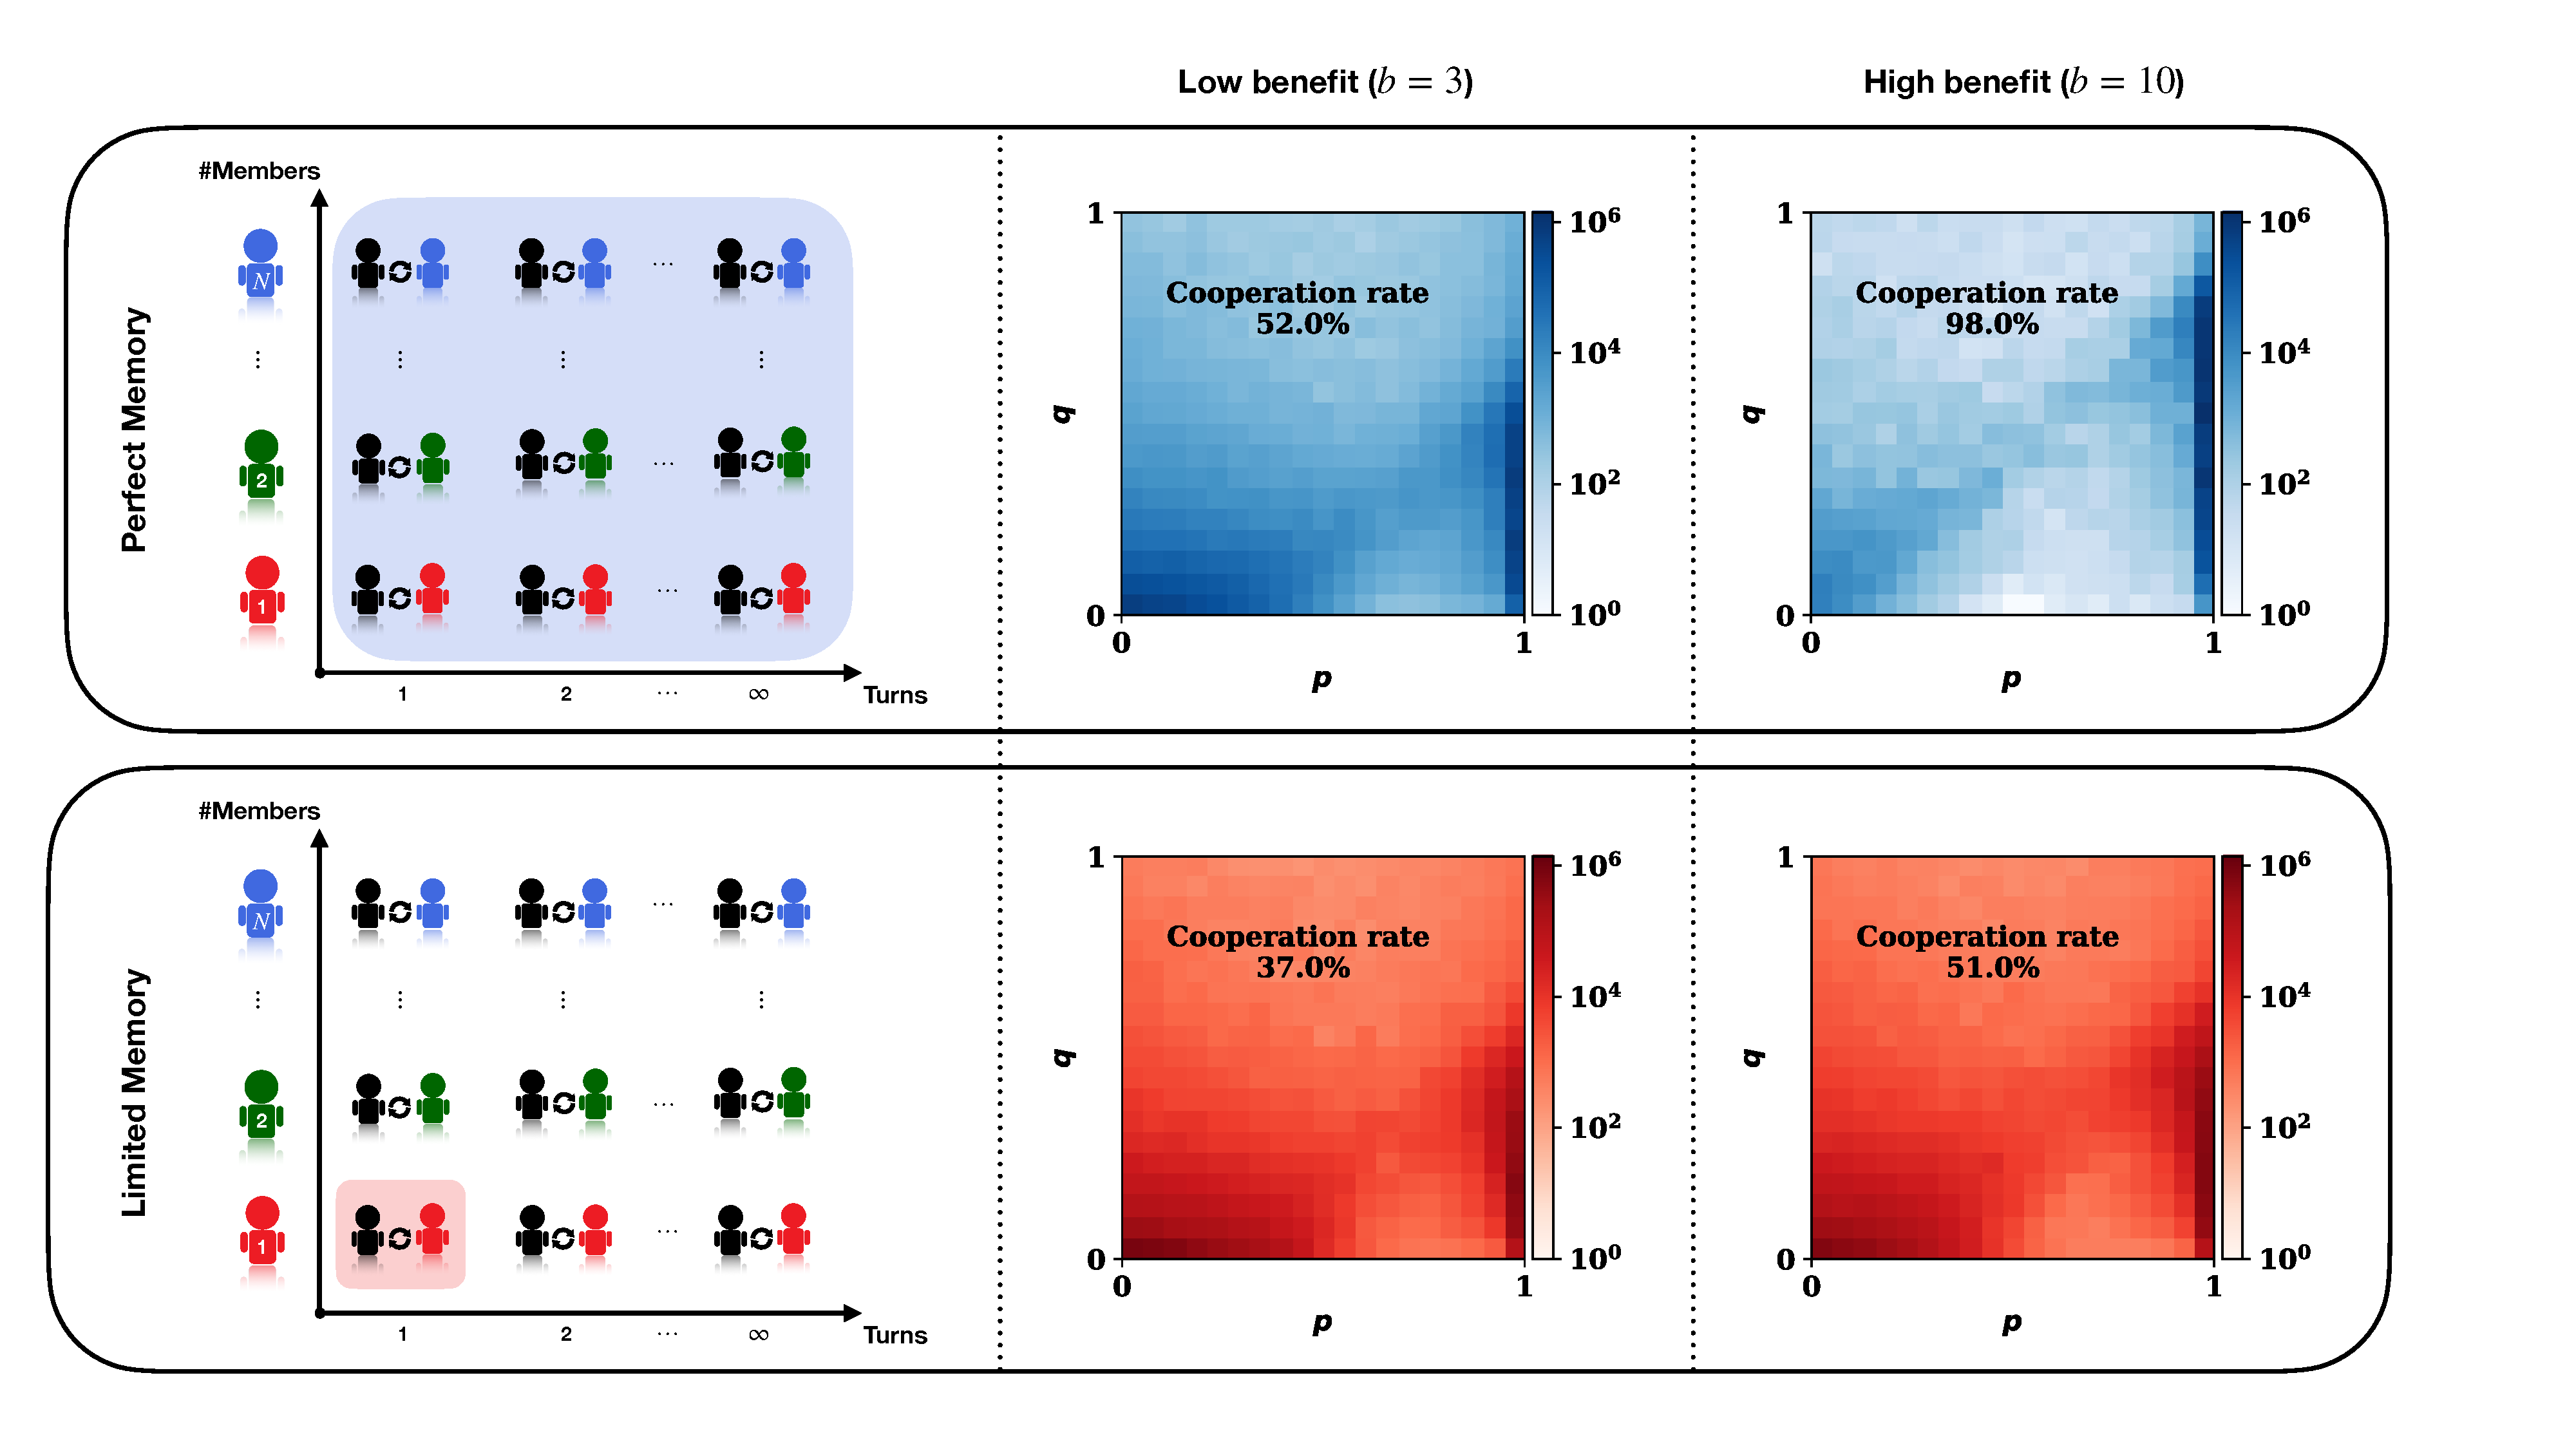
\includegraphics[width=\textwidth]{static/donation_expected_last_round_summary_results.pdf}
    \caption{{\bf Evolutionary dynamics under perfect and limited payoff memory.}
    ({\bf Schematic illustrations}) On the left panels we show schematic
    illustrations of the perfect memory and the limited memory cases. The shaded
    background denotes the game phase information that an individual considered
    when updating strategies. In the case of perfect memory the entire region is
    shaded and in the case of limited memory only one turn with a single member
    of the population. ({\bf Simulations}) We have run four simulations of the
    pairwise comparison process for $T\!=\!10^7$ time steps. For each time step,
    we have recorded the current resident population ($y,p,q$). Since
    simulations are run for a relatively high continuation probability of
    $\delta\!=\!0.999$, we do not report the players' initial cooperation
    probability $y$. The graphs show how often the resident population chooses
    each combination ($p,q$) of conditional cooperation probabilities in the
    subsequent rounds. We also report the evolved cooperation rate which is
    calculated as the average cooperation rate within the resident population.
    ({\bf Perfect Memory}) In the case of low benefit the resident population
    either consists of defectors (with $p\!\approx\!q\!\approx\!0$) or of
    conditional cooperators. Conditional cooperators, or otherwise known as
    generous tit for tat, are a set of strategies that always cooperate
    following a cooperation ($p\!\approx\!1\!$) and cooperate with a probability
    $q$ given that the co-player has defected. $q$ denotes the generosity of a
    player. The resident population applies a conditional cooperator strategy
    for which $q\!\le\!1\!-\!c/b\!=\!0.67$. This is true also for the case of
    high benefit. In this case the population mainly consists of conditional
    cooperators of the form ($p\!\approx\!1\!, q\!\le\!1\!-\!1/10\!=\!0.9$). In
    the Supplementary Information Section 2.1 we show that a conditional
    cooperator needs to be of the form ($p\!\approx\!1\!, q\!\le\!1\!-\!c/b$) to
    not be invaded by defecting strategies. A higher generosity in the
    population results in a higher average cooperation rate. The average
    cooperation rate increases from 52\% for \(b\) to 98\% for \(b=10\). ({\bf
    Limited Memory}) When players update their strategies based on their
    realized payoffs in the last round, there are two different predominant
    behaviors regardless of the benefit value. The resident population either
    consists of defectors (with $p\!\approx\!q\!\approx\!0$) or of conditional
    cooperators. The maximum level of $q$ consistent with stable cooperation is
    somewhat smaller compared to the perfect memory setting, $q\!<\!0.5$.
    Namely, in the Supplementary Information Section 2.2.1 we show that
    regardless of the value of benefit, in the case of limited payoff memory, an
    individual needs a generosity smaller of $0.5$ to repel defectors. The plots
    are fairly similar regardless of the benefit, and the evolved cooperation
    rate only slightly increases from 37\% to 51\%. Parameters: $N\!=\!100$,
    $c\!=\!1$, $\beta\!=\!1$, $\delta\!=\!0.999$.}
    \label{fig:expected_and_stochastic_for_donation}
\end{figure}

We further explore the effects of the cooperation benefit and the strength of
selection on the evolved generosity \(q\) and cooperation rate
(Figure~\ref{fig:cooperation_rate_over_benefit_and_beta}).
Figure~\ref{fig:cooperation_rate_over_benefit_and_beta}\textbf{A} suggests that
perfect memory always yields a higher cooperation rate. We observe that the
cooperation rate increases as the value of the benefit gets higher, whereas in
comparison for the limited memory payoffs, the cooperation rate remains
unchanged (as we would have expected) at approximately 50\% once \(b=5\). From
Figure~\ref{fig:cooperation_rate_over_benefit_and_beta}\textbf{B} we observe
that for weak selection, \(\beta < 1\), the two methods yield similar results,
however, as \(\beta\) increases there is variation in the evolving populations.
In the case of expected payoffs the resident populations become more cooperative
as \(\beta\) increases, whereas in the case of limited memory payoffs, the
resident populations become more defective.


\begin{figure}[!htbp]
    \centering
    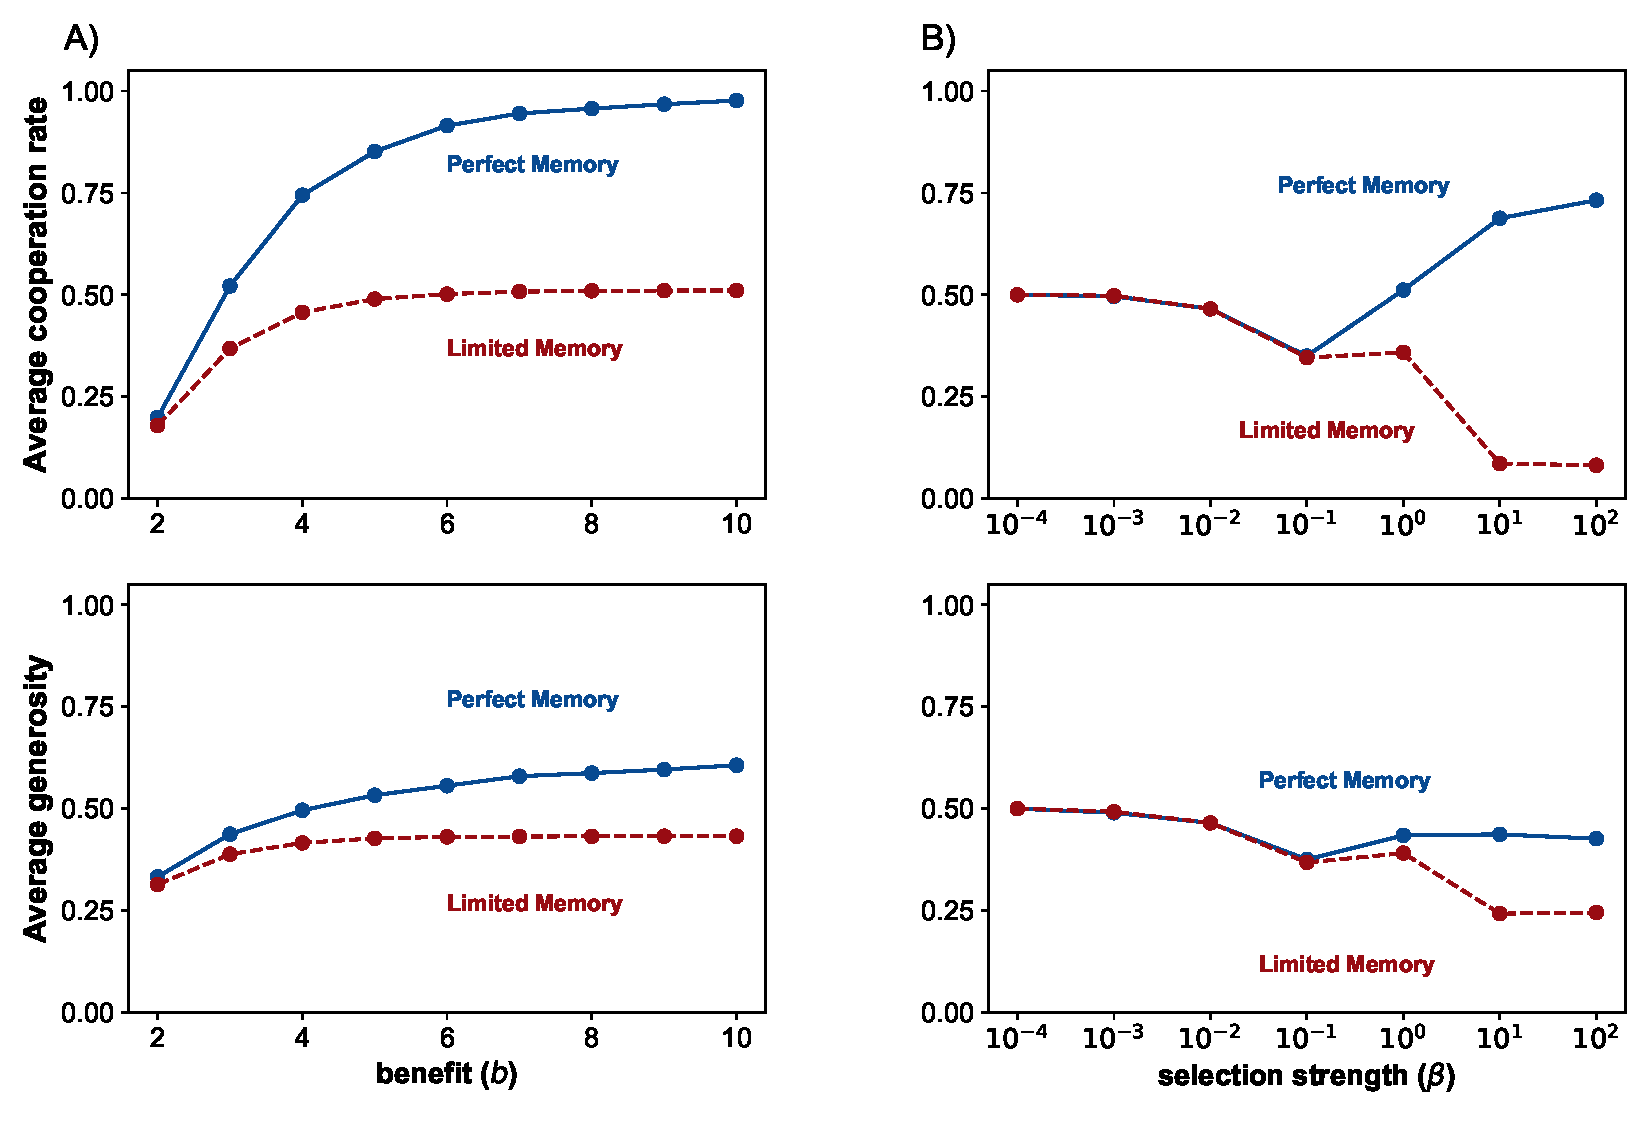
\includegraphics[width=.75\textwidth]{static/cooperation_rate_over_b_and_beta.pdf}
    \caption{{\bf The evolution of cooperation and generosity for different
    values of benefit (A) and strength of selection (B).} We report the average
    cooperation and the average reciprocity. The average cooperation rate is the
    average cooperation rate within the resident population. For the average
    reciprocity we select the residents that have a $p \approx 1$ and we take
    the average of their cooperation probability $q$. ({\bf A}) We vary the
    benefit of cooperation $b$. In all cases, perfect memory updating payoffs
    appear to overestimate the average cooperation rate the population achieves.
    As expected in the case of limited memory the average generosity over the
    different values of benefit remains the same ($q \approx 0.5$), and as a
    result so does the average cooperation. ({\bf B}) We vary the selection
    strength $\beta$. For weak selection, \(\beta < 1\), the two methods yield
    similar results. However, as \(\beta\) increases in the case of limited
    memory payoffs the resident populations become more defective. Unless
    explicitly varied, the parameters of the simulation are $N\!=\!100$,
    $b\!=\!3$, $c\!=\!1$, $\beta\!=\!1$, $\delta\!=\!0.99$. Simulations are run
    for $T\!=\!5\times 10^7$ time steps for each parameter
    combination.}\label{fig:cooperation_rate_over_benefit_and_beta}
\end{figure}

\subsection{Updating Payoffs based on More Memory}

So far we have explored the difference between the expected payoffs and the last
round payoffs. To explore further the effect of limited memory we consider three
more cases. These are the cases where the updating payoffs depend on  the last
round with two members of the population, the last two rounds with another
member of the population, and the last two rounds with two members of the
population. Similar to the last round payoff. The details of each approach can
be found in the Supplementary Information. We use numerical simulation of the
pairwise process for the various schemes. The results for low and high benefit
are shown in Figure~\ref{fig:cooperation_rate_all_updating_payoffs}.

\begin{figure}[!htbp]
  \centering
  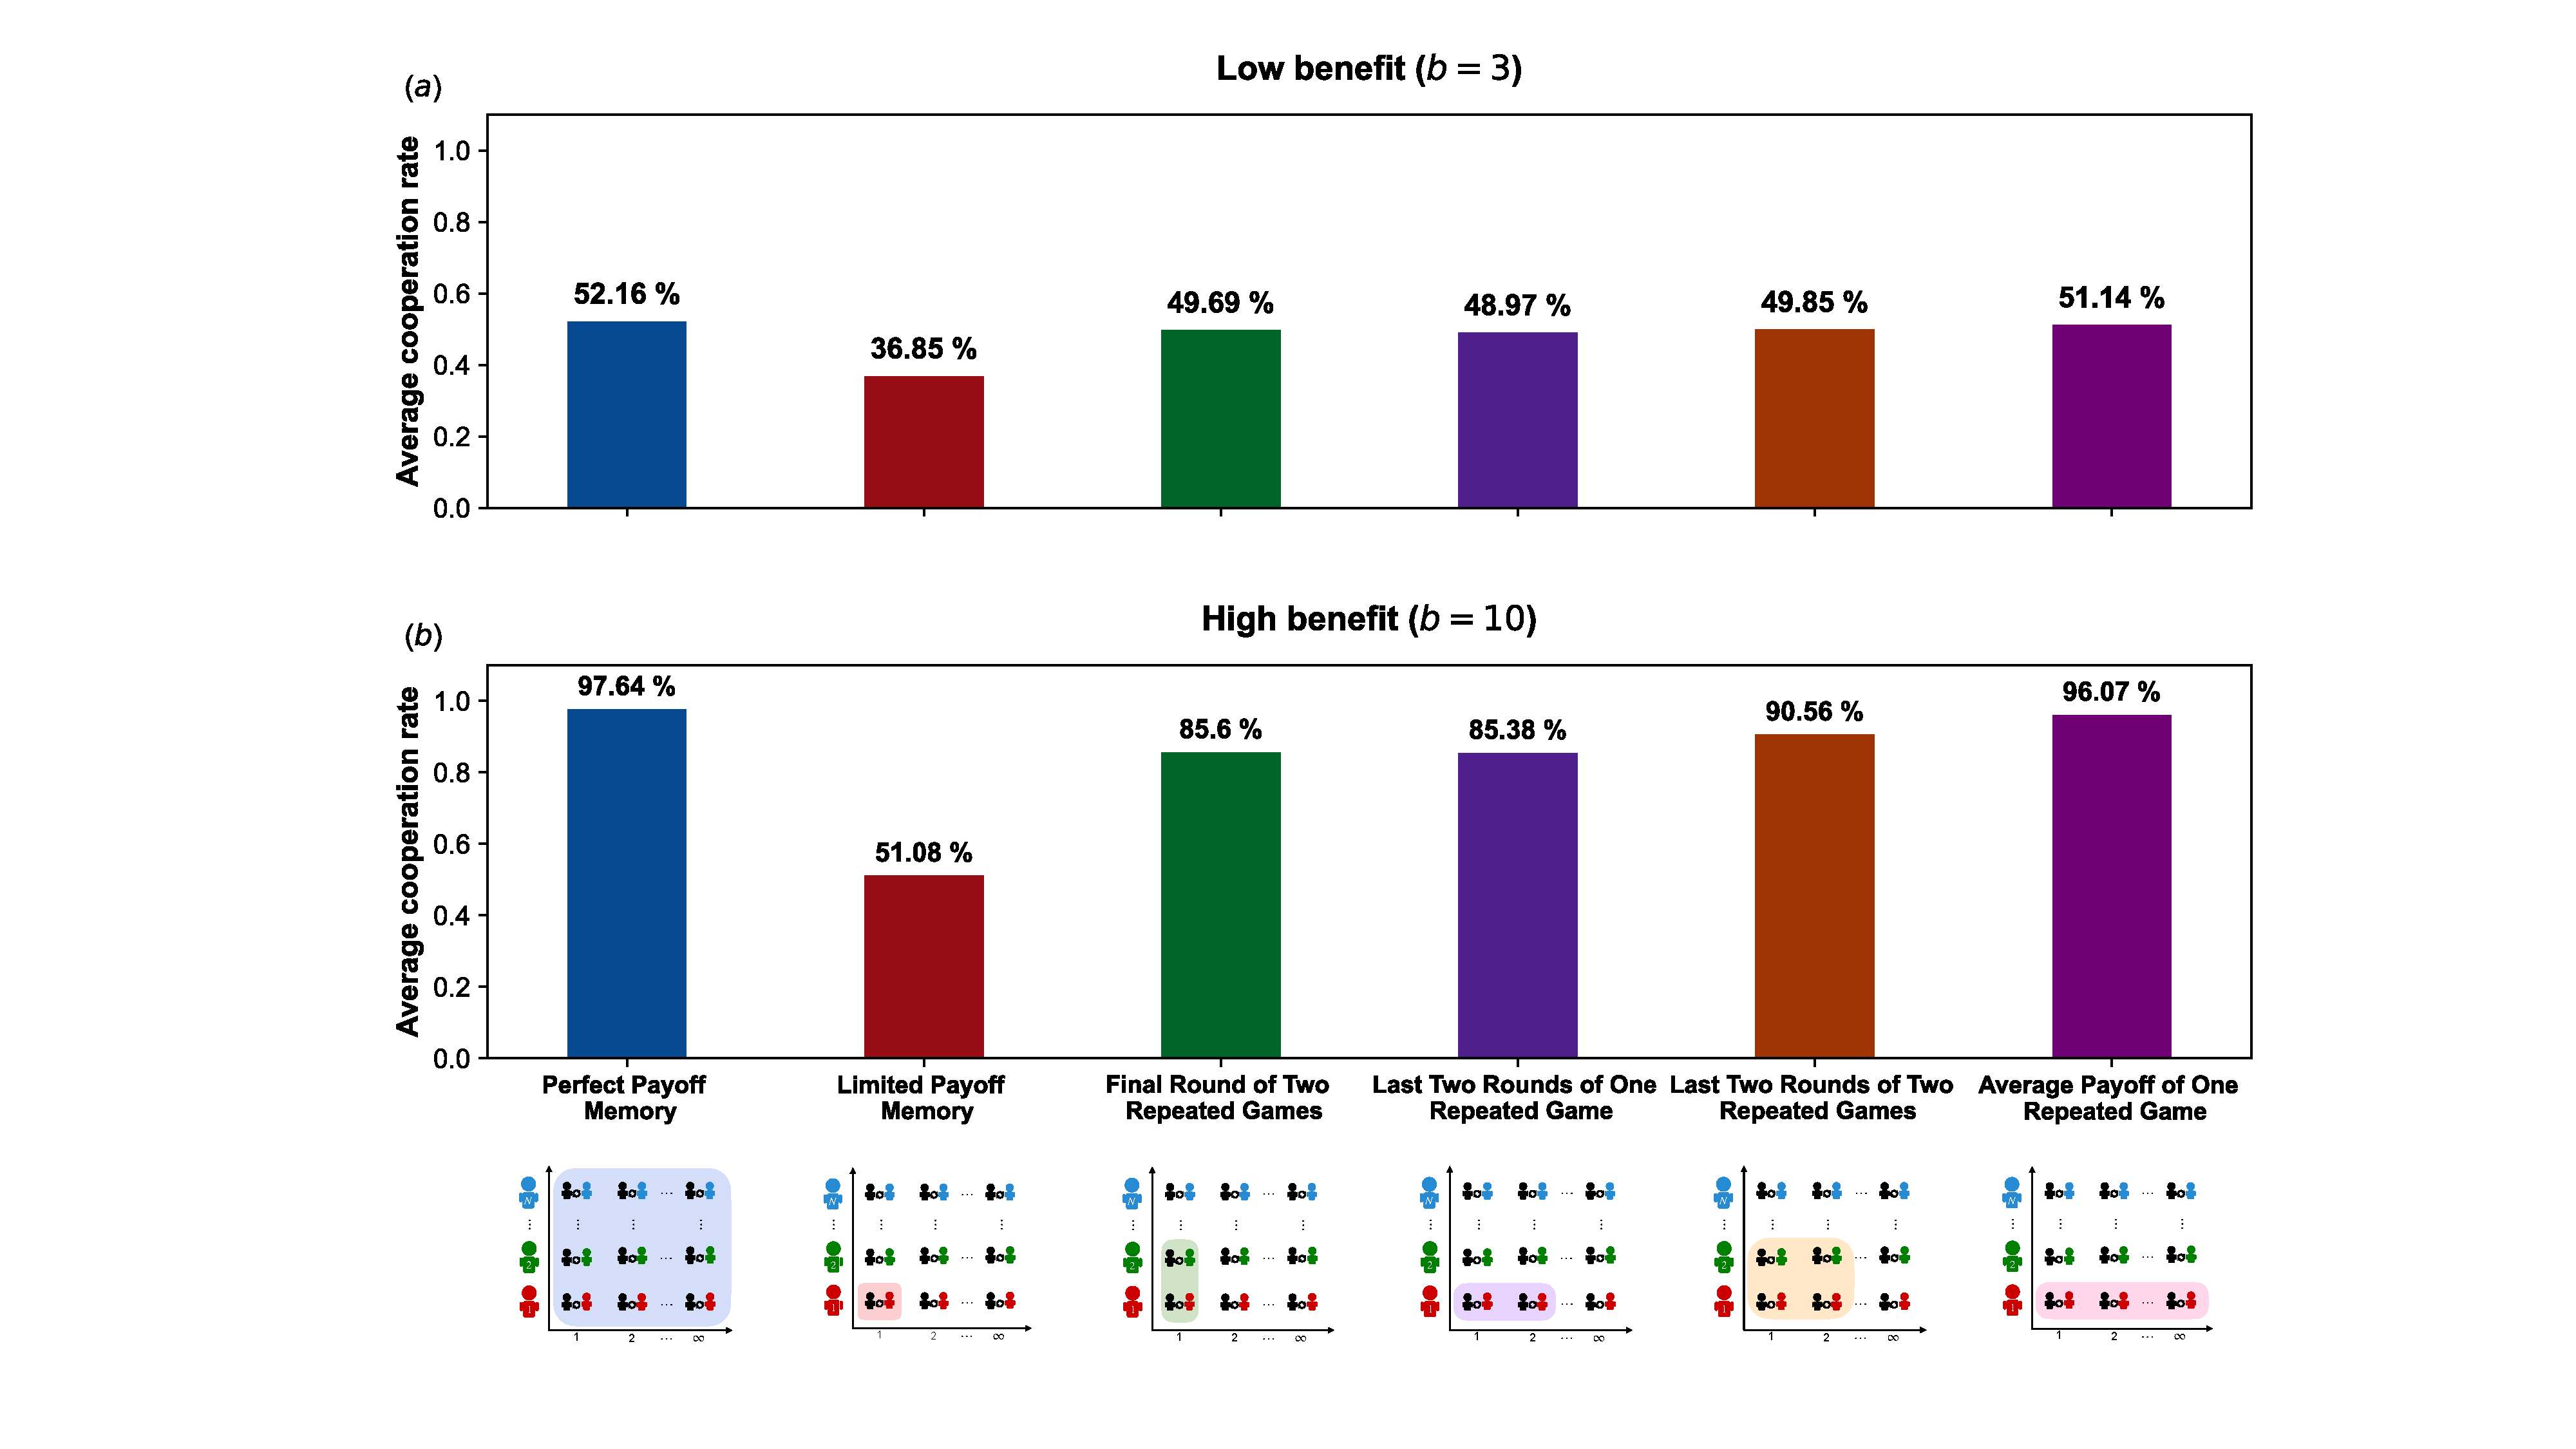
\includegraphics[width=\textwidth]{static/more_memory_summary_results.pdf}
  \caption{{\bf Average cooperation rates for different updating payoffs.}
  From left to right, we present result on the following updating payoffs cases;
  (1) the expected payoffs (perfect memory), (2) the last round payoff from one
  interaction (limited memory), (3) the last round payoff from two interactions,
  (4) the last two rounds payoffs from one interaction, (5) the last two rounds
  payoffs from two interactions. The details of each case are given in the
  Supplementary Information. Cases 3 and 4 have similar results. In that the
  evolved generosity is the same. For cases 2 - 5 the cost benefit ratio
  has an effect compared to the limited memory case. The cooperation rate
  increases, and as we allow for more information the closer we move to the
  perfect memory. Unless explicitly varied, the parameters of the simulation are
  $N\!=\!100$, $b\!=\!3$, $c\!=\!1$, $\beta\!=\!1$, $\delta\!=\!0.99$.
  Simulations are run for $T\!=\!5\times 10^7$ time steps for each parameter
  combination.}\label{fig:cooperation_rate_all_updating_payoffs}
\end{figure}

\newpage

\section{Conclusions}\label{section:conclusions}

A major focus of evolutionary game theory is the evolution of cooperation among
selfish individuals. Sometimes evolutionary game theory even seems to be reduced
to the evolution of cooperation [Arne2022]. “Why do we act altruistically to
provide a benefit to others when there is a cost to ourselves?” is still a
puzzling question amongst researchers [Glynatsi]. In this determinist
formulation, a small fraction of cooperative individuals that have a lower
fitness can never invade a population of defecting strategies.  The stochastic
effect can lead to fundamental changes since disadvantageous mutants have a
small yet non-zero probability to reach fixation in a finite population, and
thus cooperation can emerge.

Cooperation can be seen at odd, why is it that we choose to help others,
increasing their payoff, at the expense of decreasing one's own? In spite of all
the selfish genes' animal and human communities seem to altruistically help each
other and cooperate, and evolutionary game theory has helped us shape our
understanding of the evolution of cooperation.

Previous evolutionary models often feature a curious inconsistency. When
modeling how individuals make decisions in each round, these models assume that
players only remember the last round. However, when modeling how individuals
update their strategies over time, individuals are assumed to have perfect
memory.

Here, we have explored how robust cooperation is as models deviate from the
perfect memory assumption. Initially we considered the donation game. We showed
that when the last round payoff is used instead of the expected payoffs,
cooperation can even evolve when individuals only use a minimum of information,
however, the evolving cooperation rates are typically lower. The resident
strategies were both less cooperative and less generous. This effect was only
intensified we increase the benefit and the strength of selection independently.
The results showed that as each parameter was being increased the difference
between the cooperation rates were widening. This indicates that cooperative
players benefit from being able to interact with everyone in the population.

We extended our approach and presented results not only based on different
classes of social games, but also based on different limited memory payoffs. The
analysis showed that specifically for the case of the prisoner's dilemma games
the contrast between the two approaches can be significantly large. The
prisoner's dilemma is one of the most applied types of social games when we
discuss the evolution of cooperation. Our results indicate that cooperation
struggles to evolve in the prisoner's dilemma when only a minimum of social
information is used at the updating stage.

\section{Acknowledgements}

This work was supported by the European Research Council Starting Grant 850529:
E-DIRECT.


% \appendix

% \section{Model Setup}\label{appendix:methods}

% Consider a population of \(N\) individuals where \(N\) is even. At any point in
% time there are at most two different strategies in present in the population.
% More specifically, a mutant strategy played by \(k\) individuals and a resident
% strategy played by \(N - k\) individuals. We assume a pairwise process in which
% strategies spread because they are imitated more often. Each step of the
% evolutionary process consists of two stages; a game stage and an update stage.

% In the game stage, each individual is randomly matched with some other
% individual in the population. Their interaction lasts for a number of turns
% which is not fixed but depends on the continuation probability \(\delta\). At
% each turn the individuals choose between cooperation (\(C\)) and defection
% (\(D\)). Thus, there are four possible outcomes in each turn \(CC, CD, DC\) and
% \(DD\). If both players cooperate they receive the reward payoff \(R\), whereas
% if both players defect they receive the punishment payoff \(P\). If one
% cooperates but the other defects, the defector receives the temptation to
% defect, \(T\), whereas the cooperator receives the sucker's payoff, \(S\). Let
% $\mathcal{U}=\{R,S,T,P\}$ denote the set of feasible payoffs in each round, and
% let $\mathbf{u}\!=\!(R,S,T,P)$ be the corresponding payoff vector. We present
% results for various values of $\mathcal{U}$ for all the symmetric \(2 \times 2\)
% games.

% A further assumption of our model is that individuals make use of reactive
% strategies when they make decisions in each round. Reactive strategies are a set
% of strategies that take into account only the previous action of the opponent. A
% reactive strategy can be written explicitly as a vector,

% \[s=(y, p, q)\]

% where \(y\) is the probability that the strategy opens with a cooperation and
% \(p, q\) are the probabilities that the strategy cooperates given that the
% opponent cooperated and defected equivalently.

% In the updating stage, two players are randomly drawn from the population, a
% `learner' and a `role model'. The learner adopts the role model's strategy based
% on the Fermi distribution function, %ToDo add reference

% % \begin{equation} \label{Eq:rho}
% % \rho(u_{L}, u_{RM}) = \frac{1}{1\!+\! \exp^{\!-\!\beta (u_{RM}\!-\!u_{L})}}.
% % \end{equation}

% where $u_{L}\!\in\! \mathcal{U}$ is the learner's payoff, $u_{RM}\!\in\!
% \mathcal{U}$ is the role model's payoff, and $\beta\!\ge\!0$ is the strength of
% selection.

% We iterate this basic evolutionary step until either the mutant strategy goes
% extinct, or until it fixes in the population and becomes the new resident
% strategy. After either outcome, we set $k$ to $1$ and we introduce a new mutant
% strategy which is uniformly chosen from all reactive strategies at random.
% Instead of simulating each step of the evolutionary process, we estimate the
% probability that a newly introduced mutant fixes~\cite{nowak2004emergence}. This
% is defined as the fixation probability of the mutant, and the standard form is
% the following,

% \begin{equation}\label{eq:appendix_fixation_probability}
% \varphi = \frac{1}{1+\sum\limits_{i=1}^{N-1}\prod\limits_k^i \frac{\lambda^-_k}{\lambda^+_k}},
% \end{equation}

% where \(\lambda^-_k, \lambda^+_k\) are the probabilities that the number of
% mutants decreases and increases respectively.

% This process of mutation and fixation/extinction is iterated many times. The
% evolutionary process is summarized by
% Algorithm~\ref{algorithm:pairwise_comparison}.

% \begin{algorithm}[!htbp]
%   \SetAlgoLined $N \leftarrow$ population size\; $k \leftarrow 1$\; resident
%    $\leftarrow (0, 0, 0)$\; \While{ $t <$ maximum number of steps}{mutant
%    $\leftarrow$ random: $\{\emptyset \}\ \rightarrow R^3$\; fixation probability
%    $\leftarrow \varphi $\; \If{$\varphi >$ random: $i \rightarrow [0,
%    1]$}{resident $\leftarrow$ mutant;}} \caption{Evolutionary
%    process}\label{algorithm:pairwise_comparison}
% \end{algorithm}

% The aim of this work is to explore the effect of updating memory on the
% cooperation rate of the evolved population. For this reason we consider two
% different approaches when estimating the payoffs at the updating stage. The two
% approaches we consider are those of (i) the expected and (ii) the limited memory
% payoffs.

% \subsection*{Expected Payoffs}

% The expected payoffs are the conventional payoffs used in the updating
% stage~\cite{imhof2010stochastic}. They are defined as the mean payoff of an
% individual in a well-mixed population that engages in repeated games with all
% other population members.

% We first define the payoff of two reactive strategies at the game stage. Assume
% two reactive strategies $s_1\!=\!(y_1, p_1, q_1$) and $s_2\!=\!(y_2,p_2,q_2)$.
% It is not necessary to simulate the play move by move, instead the play between
% the two strategies is defined a Markov matrix \(M\),

% \begin{equation}\label{eq:transition_matrix}
%   M = \left[\begin{matrix} p_{1} p_{2} & p_{1} \left(1 - p_{2}\right) & p_{2} \left(1 - p_{1}\right) & \left(1 - p_{1}\right) \left(1 - p_{2}\right)\\
    p_{2} q_{1} & q_{1} \left(1 - p_{2}\right) & p_{2} \left(1 - q_{1}\right) & \left(1 - p_{2}\right) \left(1 - q_{1}\right)\\
    p_{1} q_{2} & p_{1} \left(1 - q_{2}\right) & q_{2} \left(1 - p_{1}\right) & \left(1 - p_{1}\right) \left(1 - q_{2}\right)\\
    q_{1} q_{2} & q_{1} \left(1 - q_{2}\right) & q_{2} \left(1 - q_{1}\right) & \left(1 - q_{1}\right) \left(1 - q_{2}\right)\end{matrix}\right].
% \end{equation}

% whose stationary vector \(\mathbf{v}\), combined with the payoff \(u\), yields
% the game stage outcome for each strategy,
% \(\langle\mathbf{v}(s_1,s_2),\mathbf{u}\rangle\)~\cite{Hauert1997}.


% In the updating stage the learner adopts the strategy of the role model based on
% their updating payoffs. Given that there are only two different types in the
% population at each time step we only need to define the expected payoff for a
% resident (\(\pi_R\)) and for a mutant (\(\pi_M\)). Assume the resident strategy
% \(s_R = (y_R, p_R, q_R)\) and the mutant strategy \(s_M = (y_M, p_M, q_M)\), the
% expected payoffs are give by,

% \begin{equation} \label{Eq:ExpPay}
%   \begin{array}{lcrcr}
%   \displaystyle \pi_R	&=	&\displaystyle \frac{N\!-\!k\!-\!1}{N-1}\cdot \langle\mathbf{v}(s_R,s_R),\mathbf{u}\rangle	&+	&\displaystyle\frac{k}{N-1}\cdot \langle\mathbf{v}(s_R,s_M),\mathbf{u}\rangle,\\[0.5cm]
%   \displaystyle \pi_M	&=	&\displaystyle\frac{N-k}{N-1}\cdot \langle\mathbf{v}(s_M,s_R),\mathbf{u}\rangle&+	&\displaystyle\frac{k-1}{N-1}\cdot \langle\mathbf{v}(s_M,s_M),\mathbf{u}\rangle.\\
%   \end{array}
% \end{equation}

% The number of mutant in the population increase if a learner resident adopts the
% strategy of a mutant role model, and decreases if a mutant leaner adopts the
% strategy of a resident. The probabilities that the number of mutants decreases
% and increases, \(\lambda^-_k\) and \(\lambda^+_k\), are now explicitly defined
% as,

% \begin{align*} 
%   \lambda^-_k &\!=\!\rho(\pi_R, \pi_M) \\
%   \lambda^+_k &\!=\!\rho(\pi_M, \pi_R).
% \end{align*}

% \subsection*{Limited memory payoffs}

% Initially, we discuss the case of the \textbf{last round updating payoff}. At
% the stage game we define the payoff of a reactive strategy in the last round,
% Proposition~\ref{proposition:last_round}.

% \begin{Prop}\label{proposition:last_round} Consider a repeated game, with
%     continuation probability $\delta$, between players with reactive strategies
%     $s_1\!=\!(y_1, p_1, q_1$)  and $s_2\!=\!(y_2,p_2,q_2)$ respectively. Then
%     the probability that the $s_1$ player receives the payoff $u\!\in\!
%     \mathcal{U}$ in the very last round of the game is given by
%     $v_{u}(s_1,s_2)$, as given by Equation~(\ref{Eq:LastRound}).

%     \begin{equation} \label{Eq:LastRound}
%       \setlength{\arraycolsep}{1pt}
%       \begin{array}{rcl}
    
%       v_{R}(s_1,s_2) &= &\displaystyle (1\!-\!\delta)\frac{y_1y_2}{1\!-\!\delta^2 r_1 r_2}+\delta \frac{\Big(q_1+r_1\big((1\!-\!\delta)y_2+\delta q_2\big)\Big) \Big(q_2+r_2\big((1\!-\!\delta)y_1+\delta q_1\big)\Big)}
%       {\displaystyle(1\!-\!\delta r_1r_2)(1\!-\!\delta^2 r_1 r_2)} \times R,\\[1cm]
    
%       v_{S}(s_1,s_2) &= &\displaystyle (1\!-\!\delta)\frac{y_1\bar{y}_2}{1\!-\!\delta^2 r_1 r_2}+\delta \frac{\Big(q_1+r_1\big((1\!-\!\delta)y_2+\delta q_2\big)\Big) \Big(\bar{q}_2+\bar{r}_2\big((1\!-\!\delta)y_1+\delta p_1\big)\Big)}
%       {\displaystyle(1\!-\!\delta r_1r_2)(1\!-\!\delta^2 r_1 r_2)} \times S,\\[1cm]
    
%       v_{T}(s_1,s_2) &= &\displaystyle (1\!-\!\delta)\frac{\bar{y}_1y_2}{1\!-\!\delta^2 r_1 r_2}+\delta \frac{\Big(\bar{q}_1+\bar{r}_1\big((1\!-\!\delta)y_2+\delta p_2\big)\Big) \Big(q_2+r_2\big((1\!-\!\delta)y_1+\delta q_1\big)\Big)}
%       {\displaystyle(1\!-\!\delta r_1r_2)(1\!-\!\delta^2 r_1 r_2)} \times T,\\[1cm]
    
%       v_{P}(s_1,s_2) &= &\displaystyle (1\!-\!\delta)\frac{\bar{y}_1\bar{y}_2}{1\!-\!\delta^2 r_1 r_2}+\delta \frac{\Big(\bar{q}_1+\bar{r}_1\big((1\!-\!\delta)y_2+\delta p_2\big)\Big) \Big(\bar{q}_2+\bar{r}_2\big((1\!-\!\delta)y_1+\delta p_1\big)\Big)}
%       {\displaystyle(1\!-\!\delta r_1r_2)(1\!-\!\delta^2 r_1 r_2)} \times P.
%       \end{array}
%     \end{equation}

% In these expressions, we have used the notation $r_i:=p_i\!-\!q_i$,
% $\bar{y}_i\!=\!1\!-\!y_i$, $\bar{q}_i:=1\!-\!q_i$, and
% $\bar{r}_i:=\bar{p}_i\!-\!\bar{q}_i=-r_i$ for $i\!\in\!\{1,2\}$.
% \end{Prop}

% \begin{proof}
% Given a play between two reactive strategies with continuation probability
% $\delta$. The outcome at turn \(t\) is given by,

% \begin{equation}\label{eq:}
%   (1 - \delta) \mathbf{v_0} \sum \delta^{t} M^{(t)},
% \end{equation}

% where $\mathbf{v_0}$ denotes the expected distribution of the four outcomes in
% the very first round, and \(1- \delta\) the probability that the game ends. It
% can be shown that,

% \begin{align*}
%   (1 - \delta) \mathbf{v_0} \sum \delta^{t} M^{(t)} & = (1 - \delta)(\mathbf{v_0} + \delta \mathbf{v_0} M + \delta^{2}\mathbf{v_0} M ^{2} + \dots )\\ 
%    & = (1 - \delta)\mathbf{v_0} (1 + \delta M + \delta^{2}M ^{2} + \dots ) \text{ using standard formula for geometric series}\\ 
%    & = (1 - \delta)\mathbf{v_0}(I_4 - \delta M)^{-1}
% \end{align*}

% where \((1 - \delta)\mathbf{v_0}(I_4 - \delta M)^{-1}\) is vector \(\in R^{4}\)
% and it the probabilities for being in any of the outcomes \(CC, CD, DC, DD\) in
% the last round. Combining this with the payoff vector \(u\) and some algebraic
% manipulation we derive to the Equation~\ref{Eq:LastRound}.
% \end{proof}

% In the updating stage we select a mutant and resident to be either the role
% model or the learner. Given that they can interact with only one other member of
% the population, they can interact either with each other or either can interact
% with another resident or with another mutant. Thus, in each updating stage there
% are five possible combinations of pairs (Figure~\ref{fig:single_pairs}).

% Given the last round payoff and possible pair combinations for a single
% interaction, we define the probability that the respective last round payoffs of
% two players \(s_1, s_2\) are given by $u_1$ and $u_2$ as,

% \begin{equation}\label{eq:Chi}
% \setlength{\arraycolsep}{1pt}
% \begin{array}{llrl}
% x(u_1,u_2)	 &=&\displaystyle \frac{1}{N\!-\!1}\cdot  &v_{u_1}(s_1,s_2)\cdot 1_{(u_1,u_2)\in \mathcal{U}^2_F}\\[0.5cm]
% &+	
% &\displaystyle \left(1\!-\!\frac{1}{N\!-\!1}\right)  
% &\left[ \frac{k\!-\!1}{N\!-\!2}\frac{k\!-\!2}{N\!-\!3} v_{u_1}(s_1,s_2) v_{u_2}(s_2,s_2) + 
%  \frac{k\!-\!1}{N\!-\!2}\frac{N\!-\!k\!-\!1}{N\!-\!3} v_{u_1}(s_1,s_2) v_{u_2}(s_2,s_1)\right.\\[0.5cm]
% &&&\left. +\frac{N\!-\!k\!-\!1}{N\!-\!2}\frac{k\!-\!1}{N\!-\!3} v_{u_1}(s_1,s_1) v_{u_2}(s_2,s_2) + 
%  \frac{N\!-\!k\!-\!1}{N\!-\!2}\frac{N\!-\!k\!-\!2}{N\!-\!3} v_{u_1}(s_1,s_1) v_{u_2}(s_2,s_1)\right].
% \end{array}
% \end{equation}

% The first term on the right side corresponds to the case that the learner and
% the role model happened to be matched during the game stage, which happens with
% probability $\frac{1}{(N\!-\!1)}$. In that case, we note that only those payoff
% pairs can occur that are feasible in a direct interaction,
% $\splitatcommas{(u_1,u_2)\in \mathcal{U}^2_F:=\big\{ (R,R), (S,T), (T,S), (P,P)
% \big\}}$, as represented by the respective indicator function. Otherwise, if the
% learner and the role model did not interact directly, we need to distinguish
% four different cases, depending on whether the learner was matched with a
% resident or a mutant, and depending on whether the role model was matched with a
% resident or a mutant.

% Given that $N\!-\!k$ players use the resident strategy
% $s_{R}\!=\!(y_{R},p_{R},q_{R})$ and that the remaining $k$ players use the
% mutant strategy $s_{M}\!=\!(y_{M},p_{M},q_{M})$, the probability that the number
% of mutants increases by one in one step of the evolutionary process can be
% written as

% \begin{align}
% \lambda^+_k=\frac{N\!-\!k}{N}\cdot \frac{k}{N}\cdot \sum_{u_{R},u_{M}\in\mathcal{U}} x(u_{R},u_{M})\cdot \rho(u_{R},u_{M}), \\
% \lambda^-_k=\frac{N\!-\!k}{N}\cdot \frac{k}{N}\cdot \sum_{u_{R},u_{M}\in\mathcal{U}} x(u_{R},u_{M})\cdot \rho(u_{M},u_{R}).
% \end{align}

% In this expression, $\frac{(N\!-\!k)}{N}$ is the probability that the randomly
% chosen learner is a resident, and $\frac{k}{N}$ is the probability that the role
% model is a mutant. The sum corresponds to the total probability that the learner
% adopts the role model's strategy over all possible payoffs $u_R$ and $u_M$ that
% the two player may have received in their respective last rounds. We use
% $x(u_R,u_M)$ to denote the probability that the randomly chosen resident
% obtained a payoff of $u_R$ in the last round of his respective game, and that
% the mutant obtained a payoff of $u_M$.

% We extend our framework to consider the case where players update their
% strategies based on the outcome of \textbf{the last two turns and based on their
% interaction with two other members of the population}. At the stage game we
% define the payoff of a reactive strategy in the last two rounds,
% Proposition~\ref{proposition:last_two_rounds}.

% \begin{Prop}\label{proposition:last_two_rounds} Consider a repeated game, with
%   continuation probability $\delta$, between players with reactive strategies
%   $s_1\!=\!(y_1, p_1, q_1$)  and $s_2\!=\!(y_2,p_2,q_2)$ respectively. Let
%   $\mathcal{\tilde{U}} = \splitatcommas{\{RR, RS, RT, RP, SR, SS, ST, SP, TR,
%   TS, TT, TP, PR, PS, PT, PP\}}$ denote the set of feasible payoffs in the last
%   two rounds, and let \(\tilde{\mathbf{u}}\) be the corresponding payoff vector.
%   Then the probability that the $s_1$ player receives the payoff $u\!\in\!
%   \mathcal{\tilde{U}}$ in the very last two rounds of the game is given by,

%   \begin{equation}
%   \langle\mathbf{\tilde{v}}(s_1,s_2),\mathbf{\tilde{u}}\rangle, \text{ where } \mathbf{\tilde{v}} \in R^{16} \text{ is given by },
%   \end{equation}
%   \begin{equation}
%     \mathbf{\tilde{v}}(s_1,s_2) = (1 - \delta) m_{a_1, a_2} \delta^2 \left[\mathbf{v_0}(I_4 - \delta M)^{-1}\right]_{a_1, a_2}, \quad  m_{a_1, a_2} \in M \ \forall \ a_1, a_2 \in \{1, 2, 3, 4\}.
%   \end{equation}
% \end{Prop}

% In the updating stage we select a mutant and resident to be either the role
% model or the learner. Given that they can interact with two other members of the
% population there are a total of twenty four possible combinations of pairs
% (Figure~\ref{fig:pissible_two_pairs}).


% Given the last two rounds payoff and possible pair combinations with two
% members, we can define the probability \(x\) that the respective last round
% payoffs of two players \(s_1, s_2\) are given by $u_1$ and $u_2$ similarly to
% Eq.~(\ref{eq:Chi}). We follow the same approach to define the rest of the
% updating payoffs. These are the updating payoffs of the last round with two
% member, and the the last two rounds payoffs with one member.

% Simulating the evolutionary process for more interactions and rounds quickly
% becomes computationally intractable. Our methodology could be extended to
% include \(n\) turns and \(m\) interactions. However, for the purpose of this
% work we explore the cases only up to two turns and two interactions.


% \section{Evolutionary dynamics under limited memory payoffs for various social
% dilemmas}\label{appendix:further_simulation_results}

% \begin{figure}[!htbp]
%   \centering
%   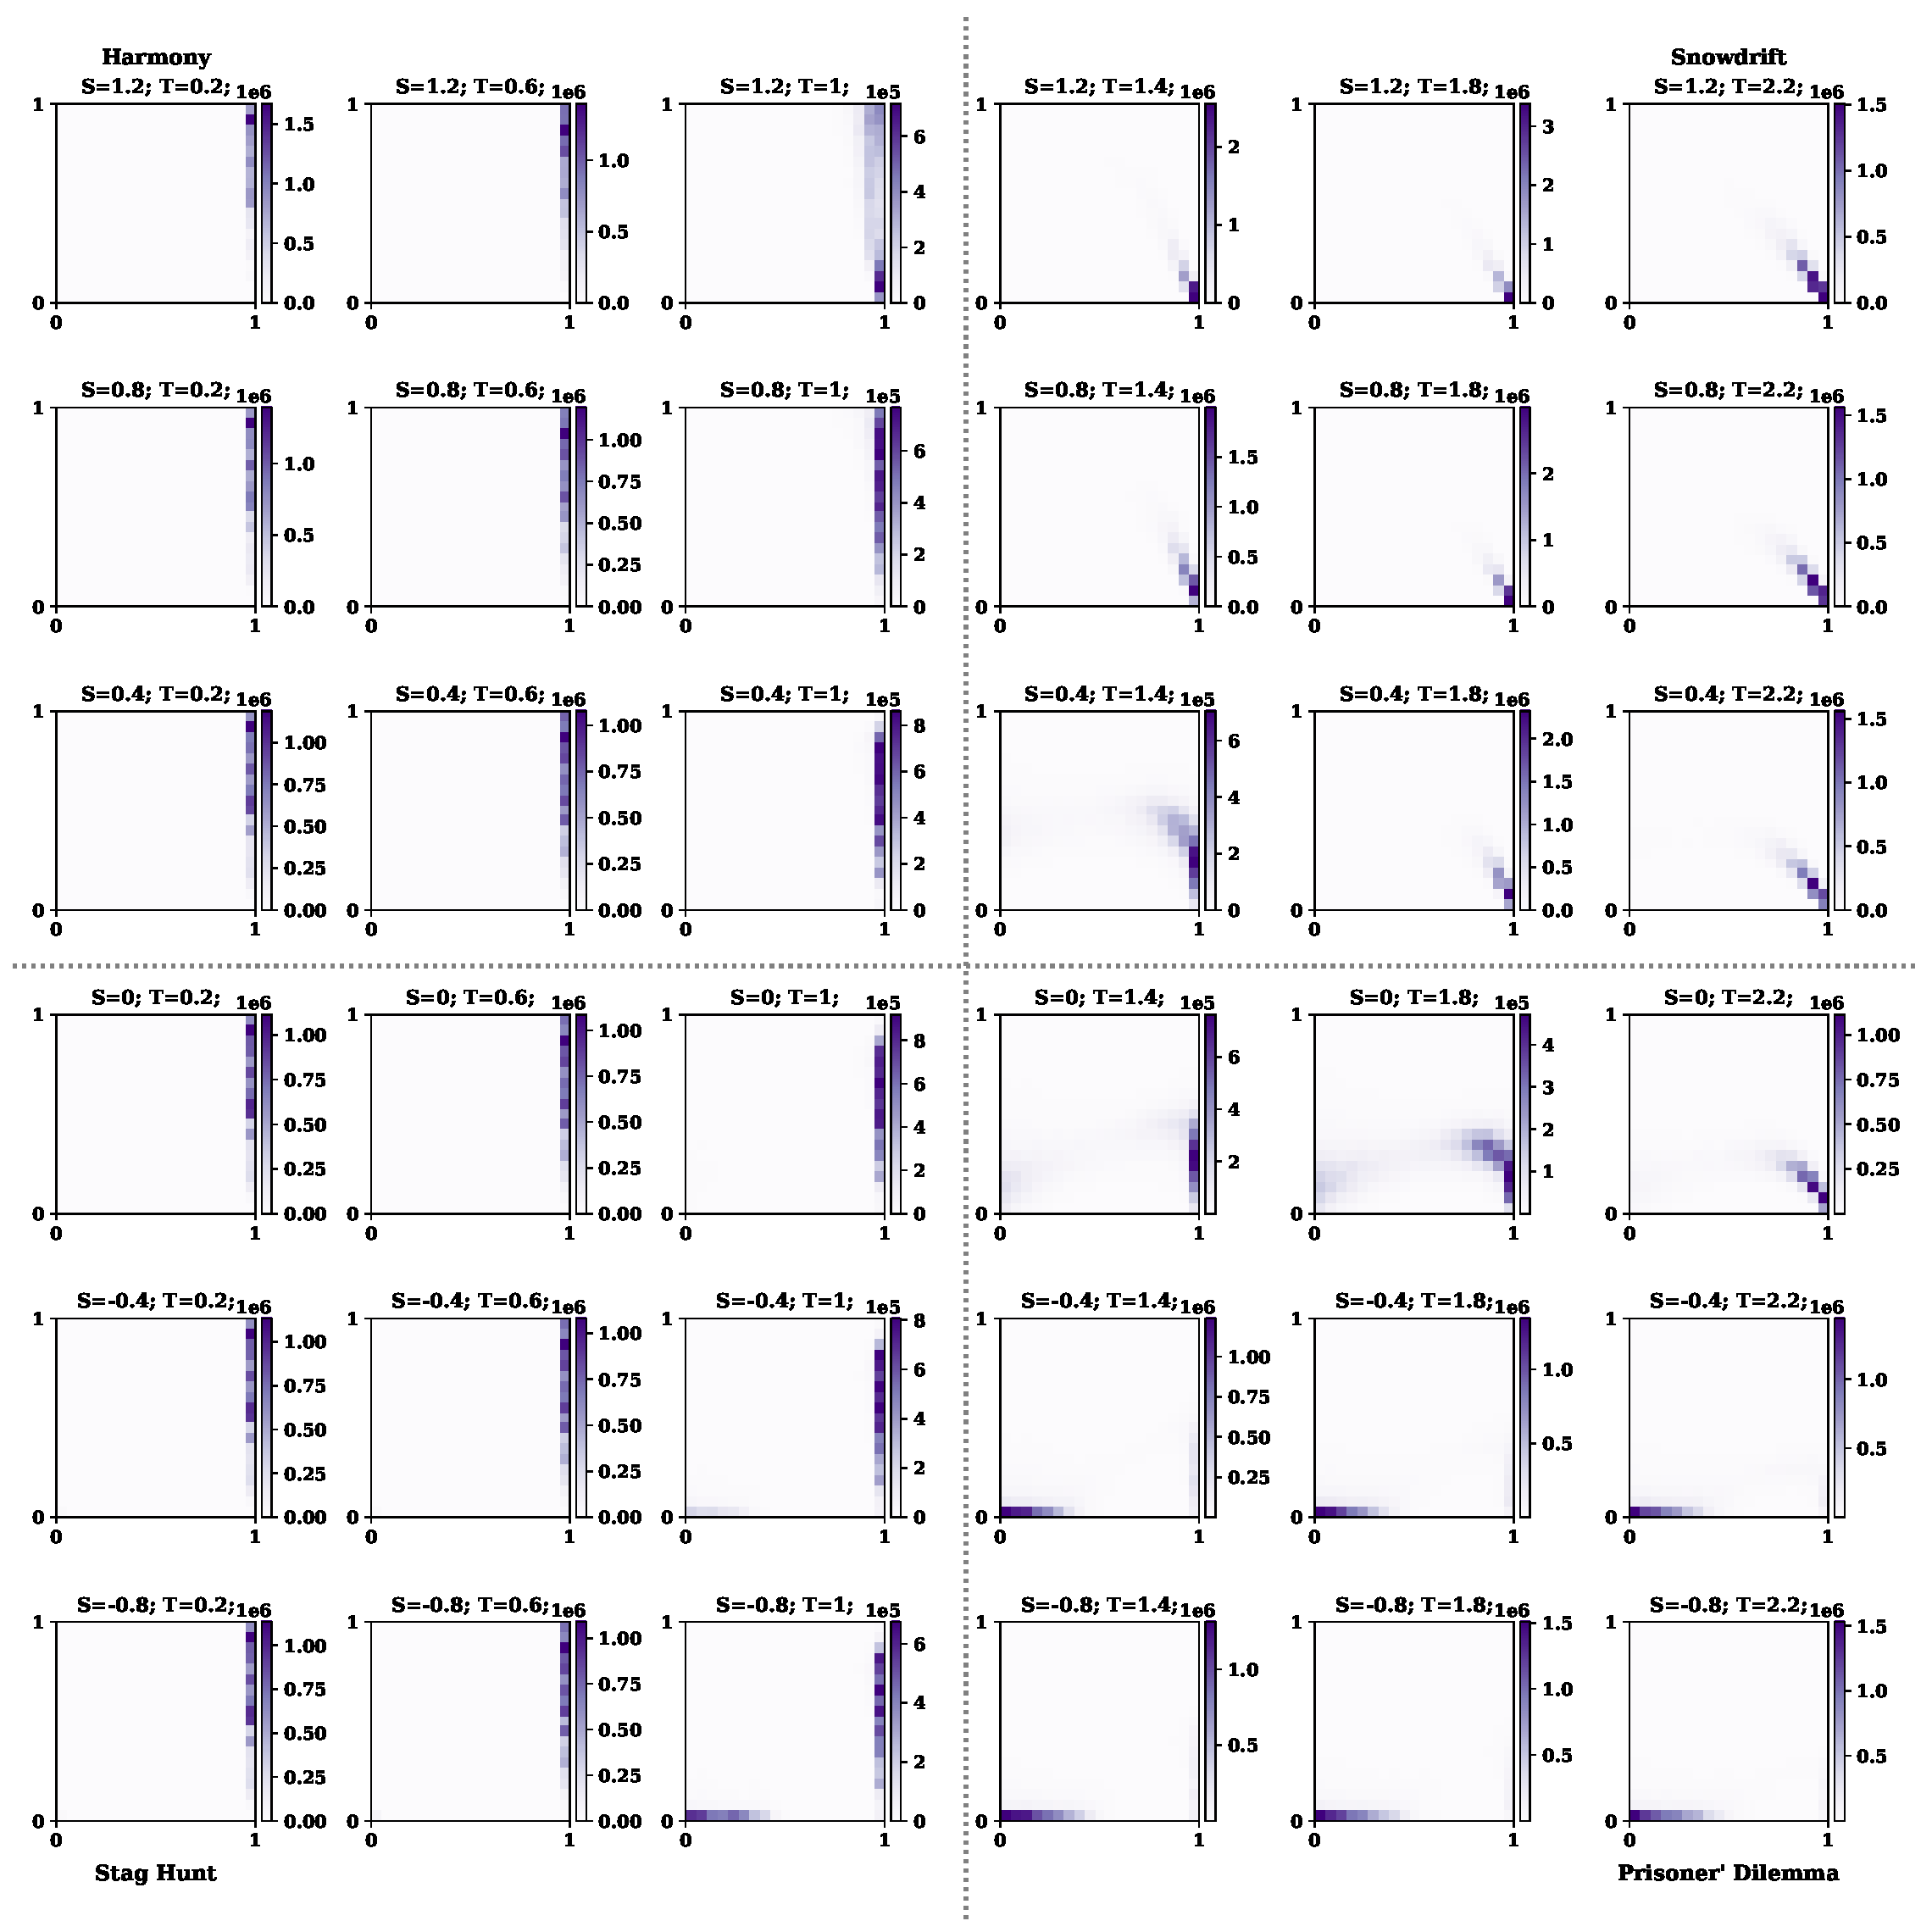
\includegraphics[width=\textwidth]{static/rounds_two_by_two_games.pdf}
%   \caption{{\bf Evolutionary dynamics under last two rounds payoffs for various social dilemmas.} 
%   We have run several simulations of the evolutionary process described in
%   section~\ref{section:model} for $t\!=\!10^7$ time steps. The graphs show how
%   often the resident population chooses each combination ($p,q$) of conditional
%   cooperation probabilities in the subsequent rounds. We vary the temptation
%   payoff \(T \in \{-1, -0.6, -0.2,  0.2, 0.6, 1, 1.4, 1.8, 2.2, 2.6, 3\}\)
%   across the \(x\) axis, and  \(S \in \{2, 1.6, 1.2, 0.8, 0.4, 0, -0.4, -0.8,
%   -1.2, -1.6, -2\}\) across the \(y\) axis. Parameters: $N\!=\!100$,
%   $\beta\!=\!10$, $\delta\!=\!0.999$.}
%   \label{fig:last_two_rounds_two_by_two}
% \end{figure}

% \begin{figure}[!htbp]
%   \centering
%   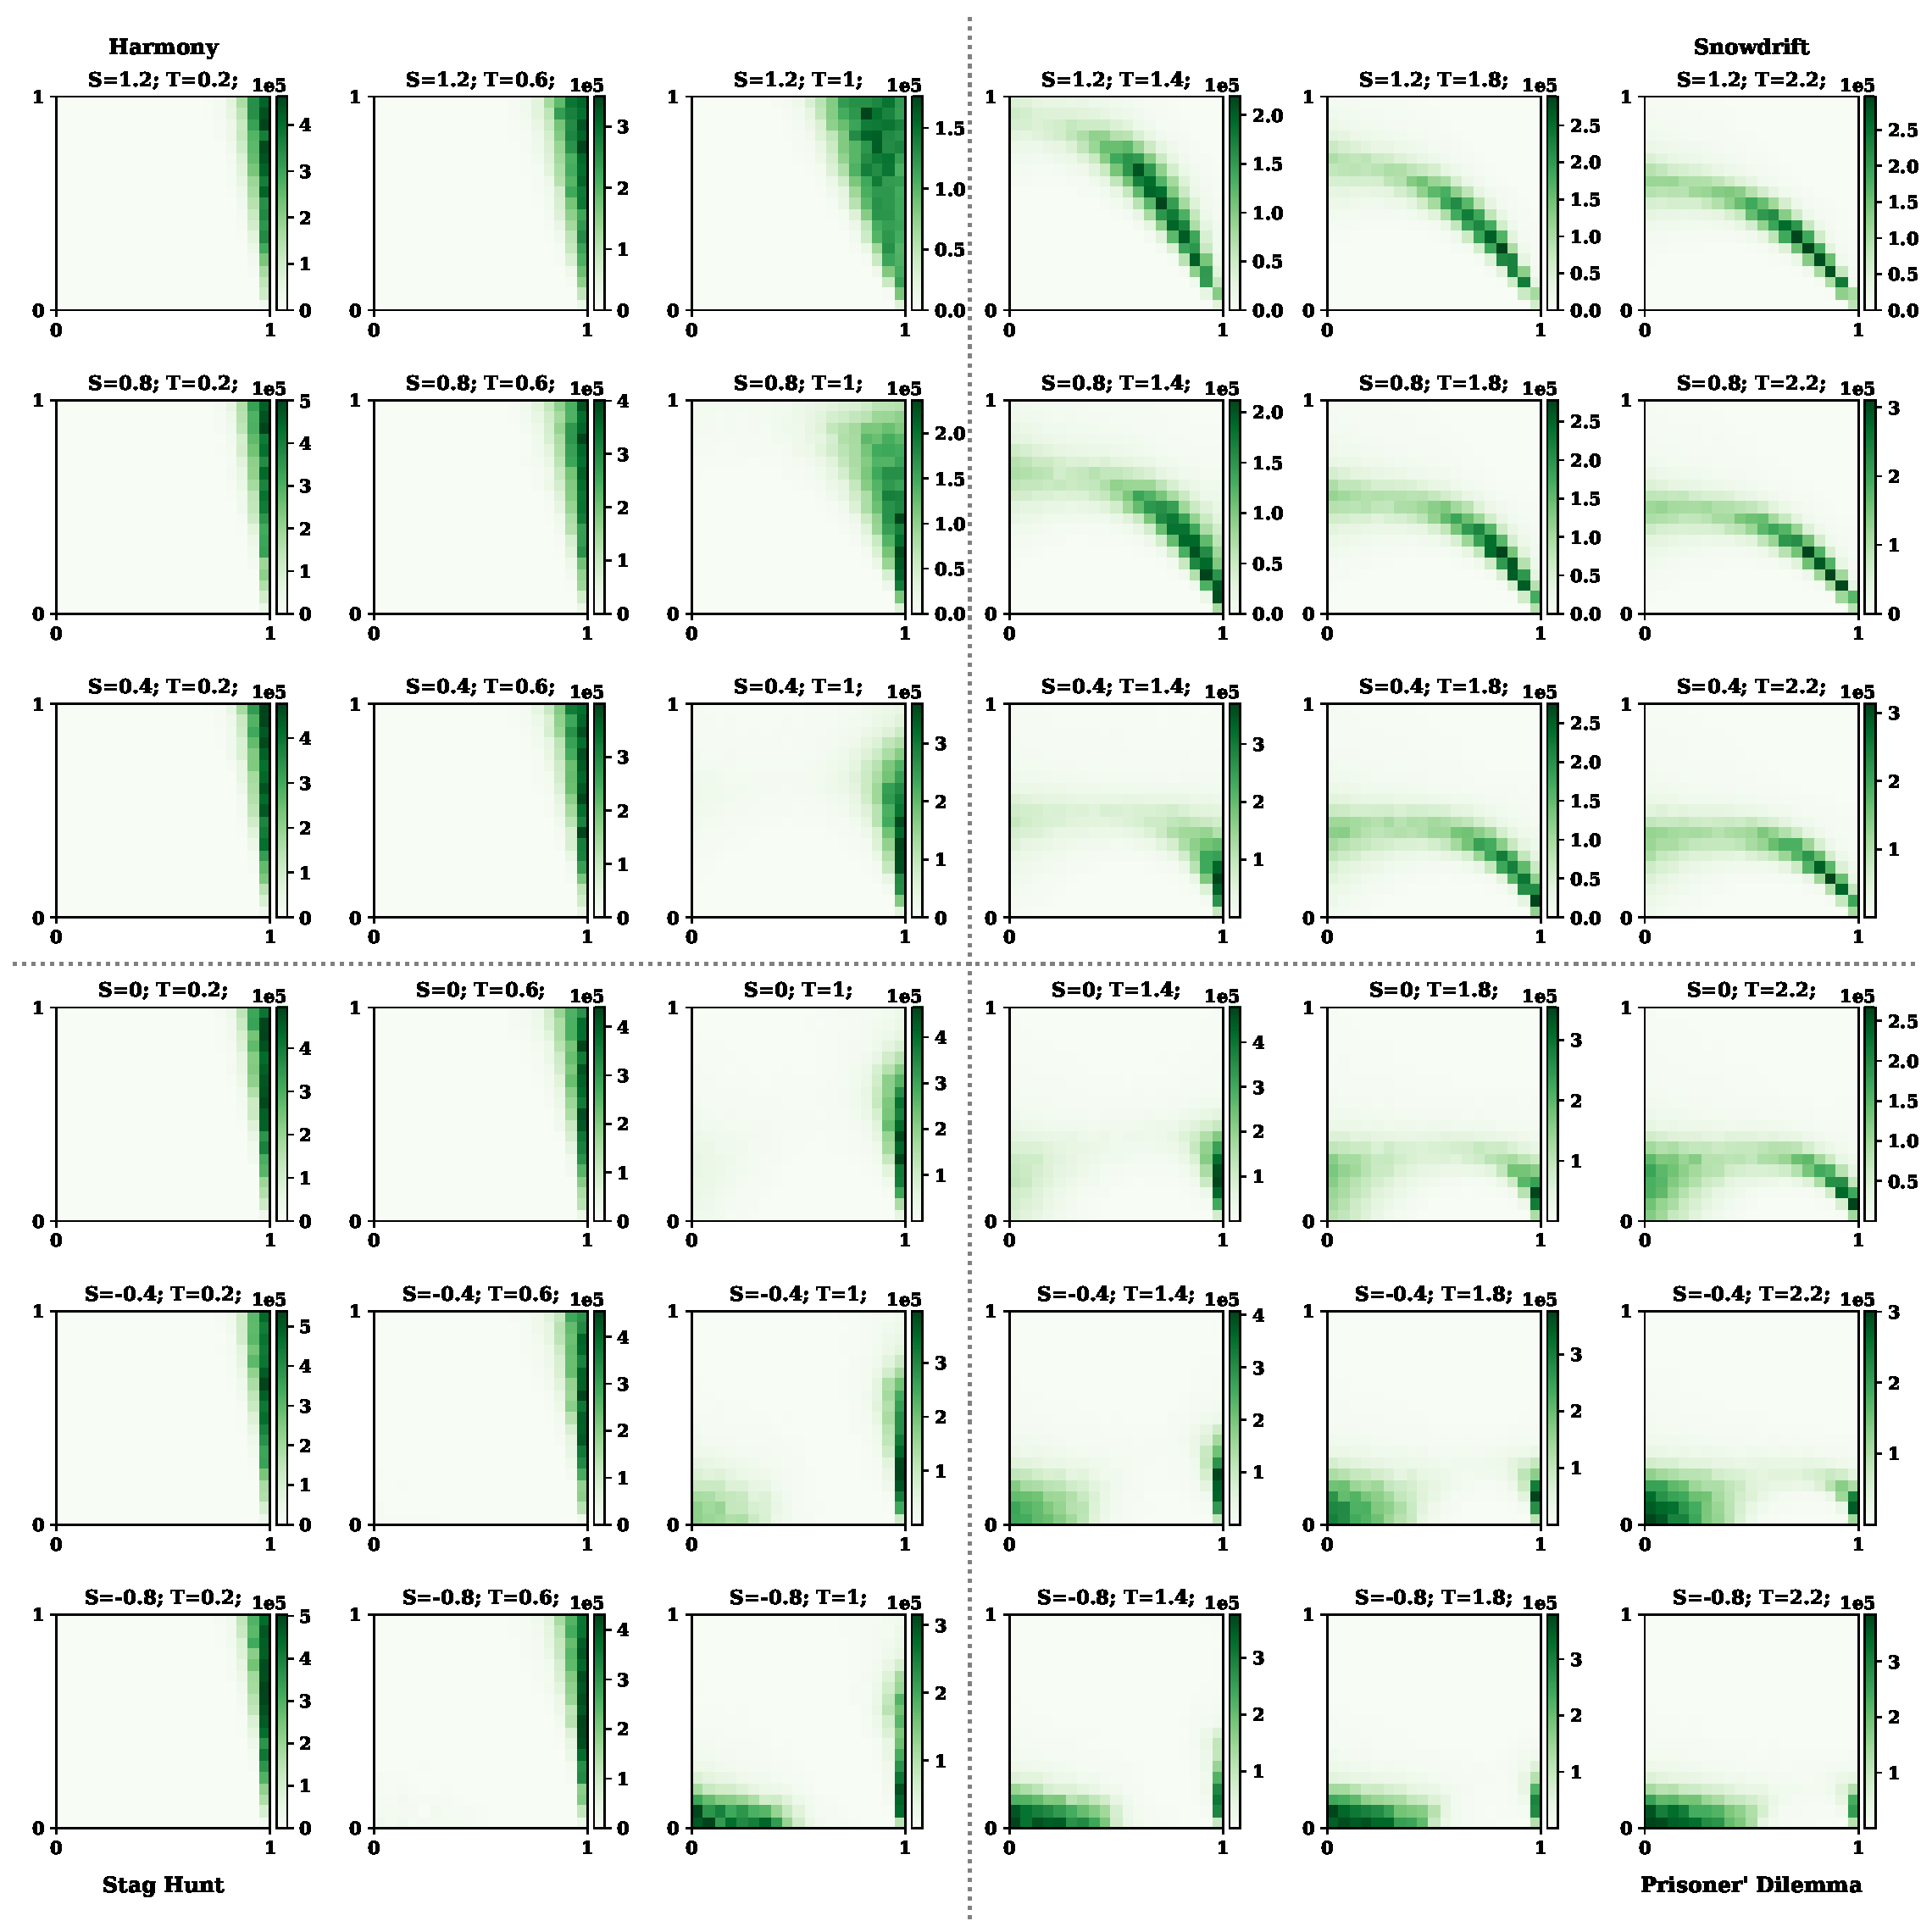
\includegraphics[width=\textwidth]{static/opponents_two_by_two_games.pdf}
%   \caption{{\bf Evolutionary dynamics under last round payoffs with two members of the population for various social dilemmas.} 
%   We have run several simulations of the evolutionary process described in
%   section~\ref{section:model} for $t\!=\!10^7$ time steps. The graphs show how
%   often the resident population chooses each combination ($p,q$) of conditional
%   cooperation probabilities in the subsequent rounds. We vary the temptation
%   payoff \(T \in \{-1, -0.6, -0.2,  0.2, 0.6, 1, 1.4, 1.8, 2.2, 2.6, 3\}\)
%   across the \(x\) axis, and  \(S \in \{2, 1.6, 1.2, 0.8, 0.4, 0, -0.4, -0.8,
%   -1.2, -1.6, -2\}\) across the \(y\) axis. Parameters: $N\!=\!100$,
%   $\beta\!=\!10$, $\delta\!=\!0.999$.}
%   \label{fig:last_two_opponents_two_by_two}
% \end{figure}

% \begin{figure}[!htbp]
%   \centering
%   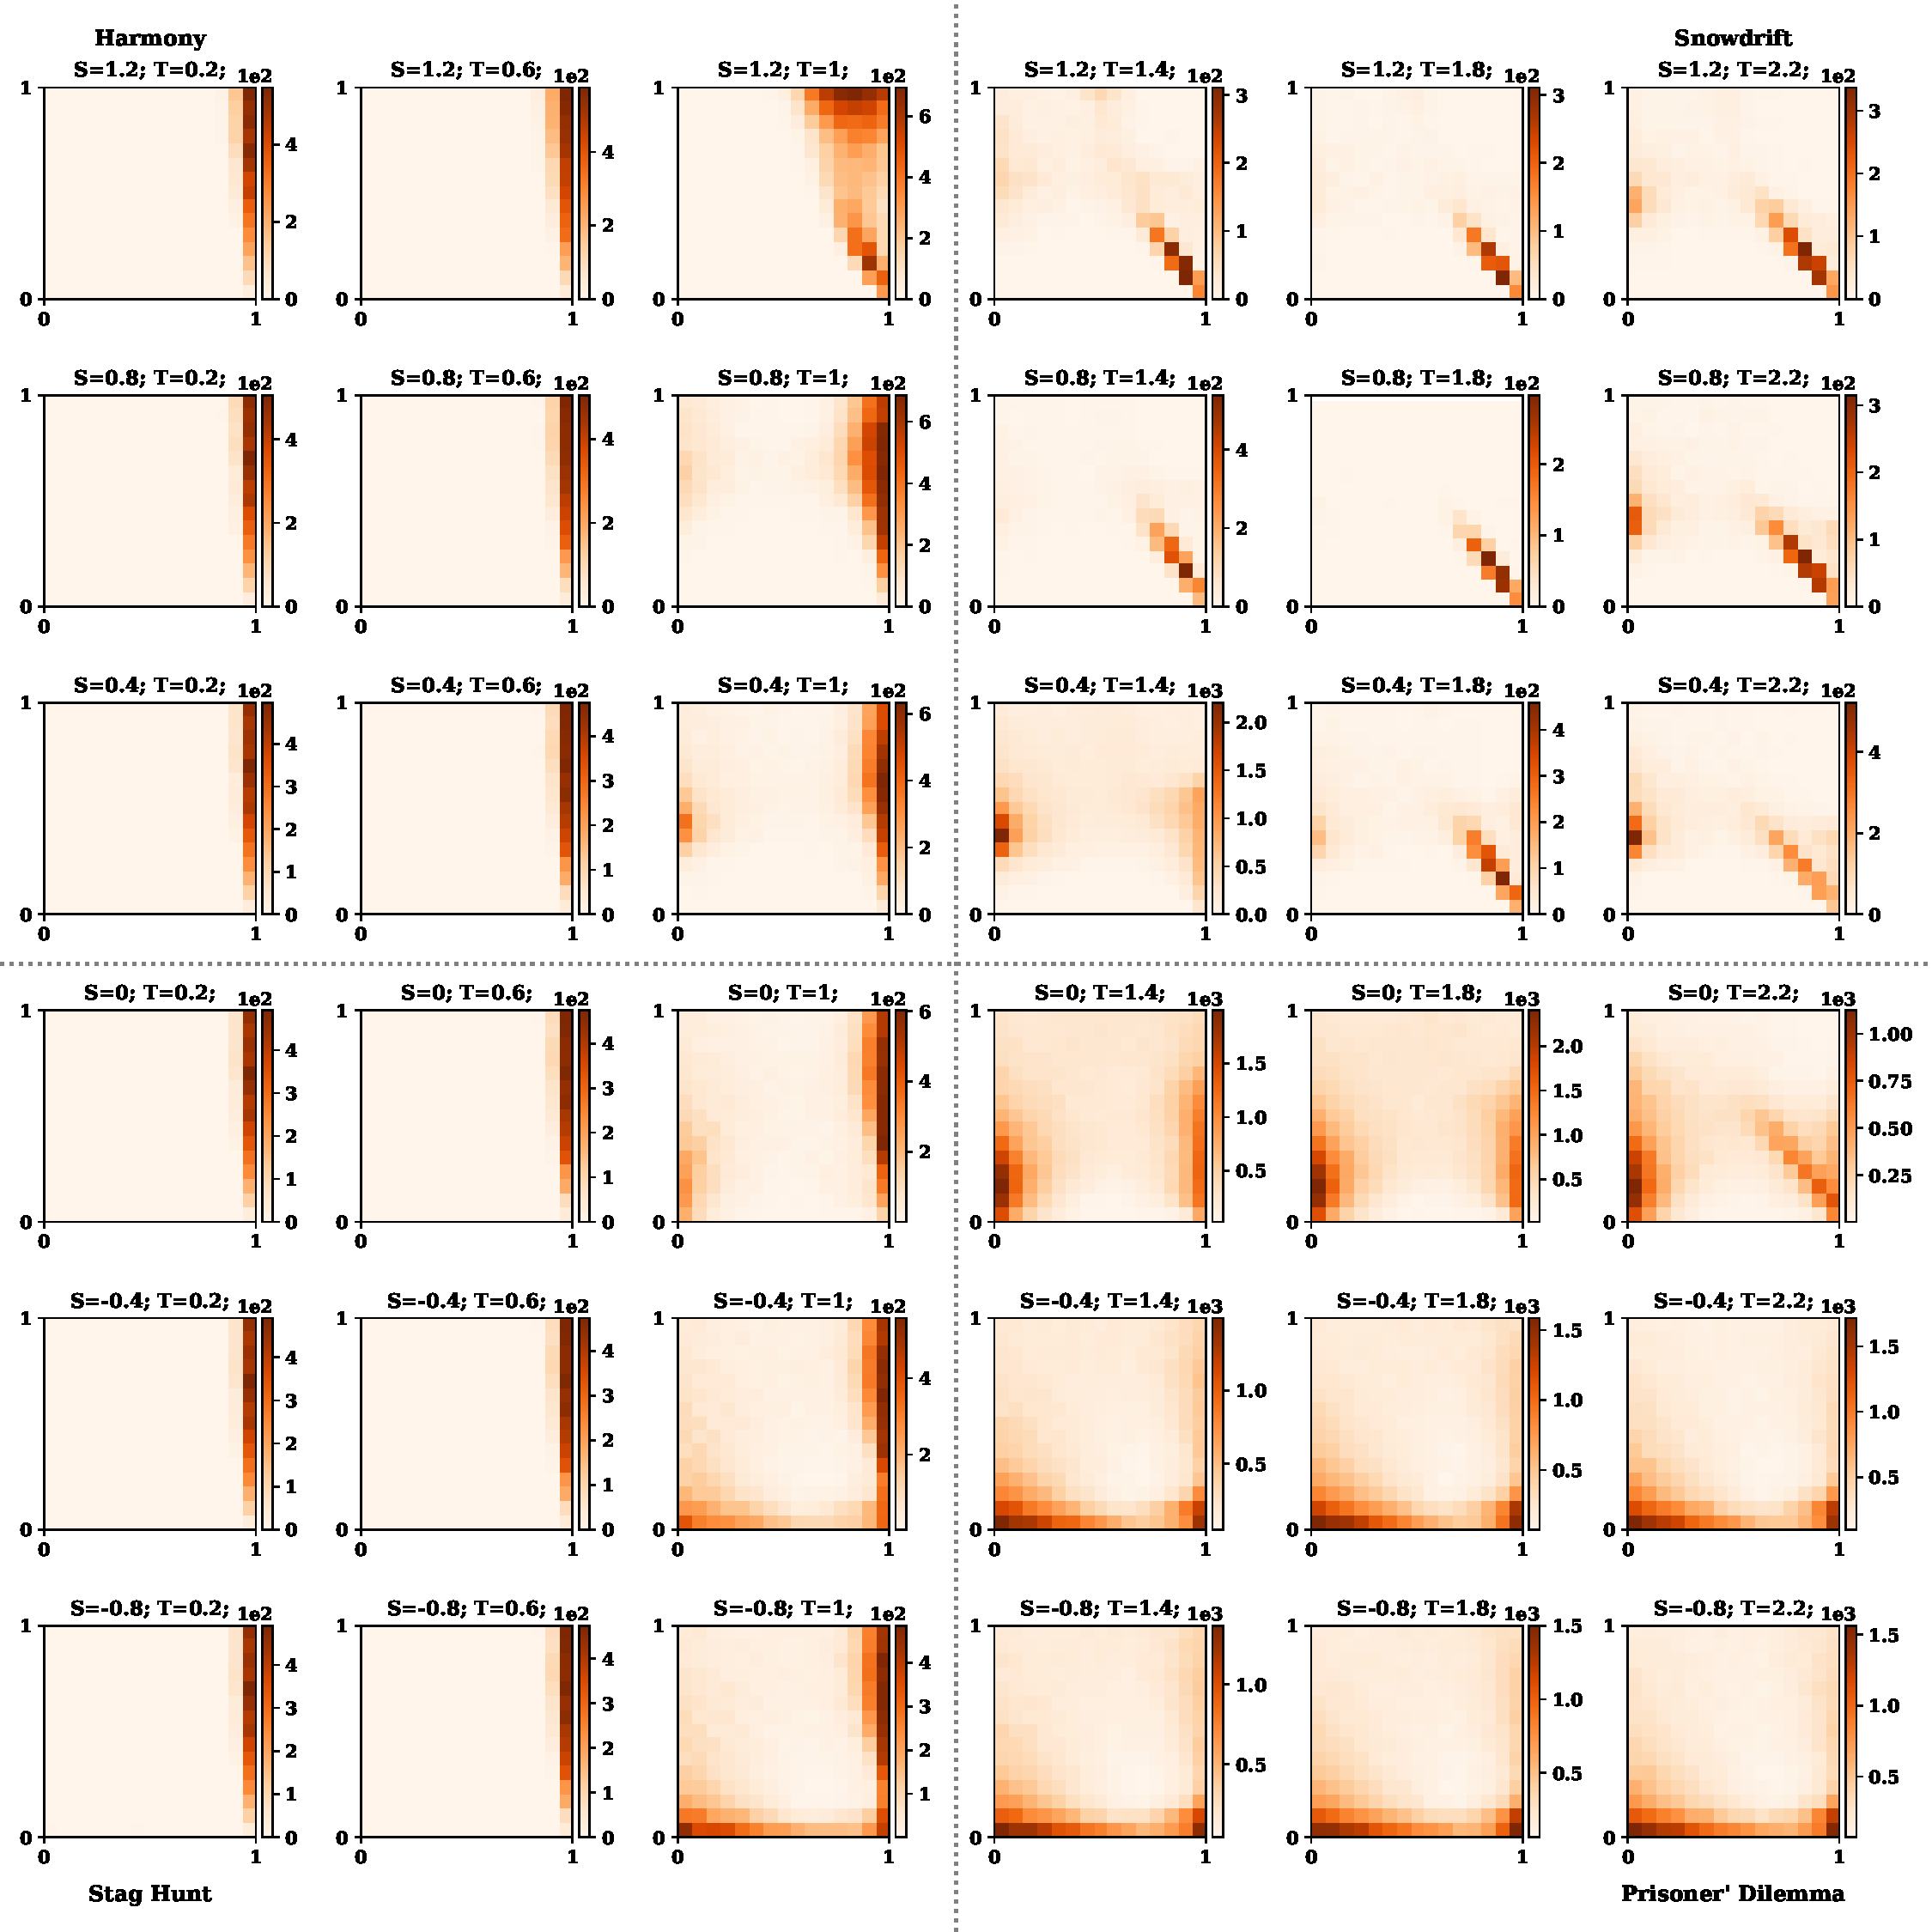
\includegraphics[width=\textwidth]{static/merged_plot_rounds_opponents_two.pdf}
%   \caption{{\bf Evolutionary dynamics under last two rounds payoffs with two members of the population for various social dilemmas.} 
%   We have run several simulations of the evolutionary process described in
%   section~\ref{section:model} for $t\!=\!10^7$ time steps. The graphs show how
%   often the resident population chooses each combination ($p,q$) of conditional
%   cooperation probabilities in the subsequent rounds. We vary the temptation
%   payoff \(T \in \{-1, -0.6, -0.2,  0.2, 0.6, 1, 1.4, 1.8, 2.2, 2.6, 3\}\)
%   across the \(x\) axis, and  \(S \in \{2, 1.6, 1.2, 0.8, 0.4, 0, -0.4, -0.8,
%   -1.2, -1.6, -2\}\) across the \(y\) axis. Parameters: $N\!=\!100$,
%   $\beta\!=\!10$, $\delta\!=\!0.999$.}
%   \label{fig:last_two_rounds_two_opponents}
% \end{figure}

\bibliographystyle{unsrt}
\bibliography{bibliography.bib}



\end{document}
